\documentclass[conference]{IEEEtran}
\IEEEoverridecommandlockouts
\usepackage{cite}
\usepackage{amsmath,amssymb,amsfonts}
\usepackage{algorithm}
\usepackage{algpseudocode}
\usepackage{graphicx}
\usepackage{textcomp}
\usepackage{xcolor}
\usepackage{booktabs}
\usepackage{multirow}
\usepackage{url}
\usepackage{tikz}
\usetikzlibrary{arrows.meta,positioning,calc,fit,shapes.geometric}
\graphicspath{{figs/}}
\pagestyle{plain}
\def\BibTeX{{\rm B\kern-.05em{\sc i\kern-.025em b}\kern-.08em T\kern-.1667em\lower.7ex\hbox{E}\kern-.125em X}}

\begin{document}

\title{Yielding, Spinning, or Both? A Simulation Study and Adaptive Hybrid Strategy for Page-Fault Handling in Microsecond-Scale Memory Disaggregation}

\author{
\IEEEauthorblockN{
  \makebox[0.3\textwidth][c]{Palem Pradeepthi}
  \makebox[0.38\textwidth][c]{Dr. N. Srinivas Naik, Ph.D.}
  \makebox[0.3\textwidth][c]{Majji Rakshitha}
}
\vspace{0.1em}
\IEEEauthorblockA{
  \makebox[0.3\textwidth][c]{\textit{Student Author}}
  \makebox[0.38\textwidth][c]{\textit{Associate Professor (Guided by)}}
  \makebox[0.3\textwidth][c]{\textit{Student Author}}
}
\vspace{0.4em}
\IEEEauthorblockA{\textit{Department of Computer Science and Engineering, IIITDM Kurnool, Kurnool, India}}
}

\maketitle

\begin{abstract}
Paging-based memory disaggregation splits application memory across local DRAM and remote memory servers over RDMA. Remote page faults take merely 2--3~$\mu$s. Because traditional OS context switches take tens of microseconds, prior disaggregation systems make faulting threads spin-poll on RDMA completion queues. The EuroSys '25 Adios paper challenges this spinning design, showing that busy-waiting causes severe head-of-line blocking and starves the RDMA link. Adios argues that ultra-fast user-level threading makes yielding viable again. Here, we build a SimPy-based discrete-event simulator to test this scheduling thesis independently of complex kernel drivers. Modeling eight worker threads, dedicated queue pairs, and a shared 100~GbE link, we evaluate busy-waiting against round-robin and page-fault-aware yielding. At a 20\% hit rate, yielding boosts saturation throughput from 1.77 to 2.50~MRPS (a $1.41\times$ improvement) and cuts P99.9 latency at 1.5~MRPS from 17.2 to 8.9~$\mu$s, matching our closed-form analytical capacity bounds within 3\%.

Going beyond the paper, our simulations reveal an overlooked trade-off: yielding adds an unavoidable latency penalty at low load where cores sit idle, and collapses if context switching exceeds half a fetch time. We therefore propose and implement an adaptive hybrid policy. By checking local inbox queues and core availability upon a fault, workers spin when the system is uncongested and yield only when queue backlog forms. This adaptive strategy matches busy-waiting's 5.30~$\mu$s median latency at light load, reaches the 2.50~MRPS saturation plateau under heavy load, and stays robust even if switch costs rise to 1.5~$\mu$s.
\end{abstract}

\begin{IEEEkeywords}
memory disaggregation, page fault handling, RDMA, tail latency, discrete-event simulation, user-level threads, unikernel, adaptive scheduling, hybrid polling
\end{IEEEkeywords}

\section{Introduction}
Modern cloud datacenters suffer from an inherent resource mismatch: compute and memory needs rarely scale in lockstep. Many servers run out of CPU cores while gigabytes of local DRAM remain untouched, while adjacent nodes hit memory exhaustion despite largely idle processors. Paging-based memory disaggregation solves this stranded-resource problem. Compute blades keep a small working set of hot pages in local memory and access the remaining pool across dedicated memory nodes over fast interconnects like RDMA.

Operating-system-level paging makes disaggregation especially practical because unmodified binaries can execute without source code changes or specialized runtime libraries \cite{infiniswap,fastswap,hermit,dilos}. Whenever a thread accesses a missing page, the hardware traps into a page fault, and the kernel issues a 4~KiB one-sided RDMA read. On modern 100~Gb/s adapters, remote reads finish in 2--3~$\mu$s. While this is orders of magnitude faster than spinning disks or solid-state storage, it sits squarely in the ``killer microsecond'' regime described by Barroso et al.\ \cite{killer}. In such latency-critical services, tail latency (P99 and P99.9) dictates user experience far more than mean response time \cite{tail,tales}.

The core dilemma during a microsecond page fault is how to handle the CPU while waiting for the network. System builders have traditionally chosen between two extremes:
\begin{enumerate}
\item \emph{Yielding the CPU}: Stash thread registers, hand the processor to another runnable task, and wake the original thread upon packet arrival. Infiniswap pioneered this in Linux \cite{infiniswap}, but kernel context switches and interrupt processing add tens to hundreds of microseconds, completely swamping the 3~$\mu$s fetch.
\item \emph{Spinning (Busy-waiting)}: Keep the core in a tight loop polling the RDMA completion queue until the page arrives. Fastswap, Hermit, and DiLOS adopt this strategy \cite{fastswap,hermit,dilos}. While busy-waiting eliminates context-switch overhead and yields low latency when load is light, it leaves cores burning power doing zero useful computation.
\end{enumerate}

The recent EuroSys '25 paper on Adios \cite{adios} revisits this trade-off. Profiling DiLOS under realistic workloads, Yoon et al.\ exposed two fatal flaws of busy-waiting under load. First, arriving requests queue up behind spinning workers and stall for the full remote fetch time---inducing severe head-of-line (HOL) blocking that balloons tail latency. Second, because each spinning thread issues only one fetch at a time, eight workers can generate at most eight concurrent requests, leaving 100~GbE links half-utilized. Adios solves this by combining unikernel zero-privilege switching, 40-cycle user-level unithreads, and congestion-aware load balancing, achieving up to $1.64\times$ throughput and $10.89\times$ P99.9 latency cuts over DiLOS \cite{adios}.

Since building a bare-metal unikernel and RDMA testbed is outside the scope of an academic term project, we study the core question: \emph{How much of Adios's gain stems strictly from the scheduling policy once context-switch cost is fixed?} To answer this, we developed a discrete-event simulator in Python (using SimPy) that models an 8-core compute node, per-worker queue pairs, and a shared 100~GbE link. We validate our simulation against exact closed-form capacity equations across diverse hit rates, cache configurations, and context-switch latencies.

Furthermore, our profiling uncovers two key weaknesses in pure yielding: (1) under low request rates, yielding adds an unnecessary 20~ns context-switch tax while peer cores sit idle, and (2) if context switches take longer than half an RDMA fetch ($t_s > 1.5~\mu$s), pure yielding collapses below spinning throughput. To fix both problems, we implement an adaptive hybrid policy that spin-waits when cores are idle and yields immediately when queue backlog forms.

\subsection*{Summary of Contributions}
\begin{itemize}
\item \textbf{Open-source simulator}: We developed a discrete-event simulator modeling queue pairs, NIC serialization, and worker scheduling, comparing spinning and yielding under identical networking constraints.
\item \textbf{Analytical capacity bounds}: We derive closed-form formulas for saturation throughput ($\Lambda_{bw}, \Lambda_{cpu}, \Lambda_{link}$) that match our simulation measurements within 3\%.
\item \textbf{Break-even condition}: We prove and verify that yielding improves capacity if and only if two context switches cost less than one remote page fetch ($2t_s < t_f$).
\item \textbf{Comprehensive parameter sweeps}: We evaluate tail latency (P99.9), carried throughput, Zipf-skewed LRU caching, and congestion-aware dispatching against published Adios data.
\item \textbf{Adaptive hybrid policy}: We introduce a queue-aware hybrid scheduling rule that eliminates light-load yielding overhead (achieving 5.30~$\mu$s median latency) while maintaining full 2.50~MRPS saturation throughput and complete resilience to switch costs up to 1.5~$\mu$s.
\item \textbf{Methodological analysis}: We detail two subtle simulation measurement bugs (arrival-time windowing and unbounded in-flight queues) and explain how analytic bounds helped us detect and correct them.
\end{itemize}

\subsection*{Scope}
Our project is deliberately scoped to simulation. We do not run bare-metal OSv unikernels or physical Mellanox NICs. Factors like kernel memory allocators, page-table locks, and reclaimer threads are omitted to isolate the pure scheduling trade-off. Our results serve to explain the underlying queuing dynamics and identify break-even thresholds rather than benchmark real hardware.

\subsection*{Paper Outline}
The report is structured as follows. Section~\ref{sec:background} covers disaggregation fundamentals and waiting strategies. Section~\ref{sec:related} discusses related work. Section~\ref{sec:adios} reviews Adios's key mechanisms and published figures. Section~\ref{sec:model} presents our simulation model and capacity bounds. Section~\ref{sec:method} describes our experimental methodology. Section~\ref{sec:results} presents our findings, including the adaptive hybrid policy. Section~\ref{sec:analysis} uses the validated models for analytical extrapolation. Section~\ref{sec:discussion} discusses threats to validity, and Section~\ref{sec:conclusion} concludes.

\section{Background}
\label{sec:background}

\subsection{Disaggregated memory and paging}
In a disaggregated deployment, the compute node holds only a portion of the memory that its applications actually address---perhaps one fifth of the total working set---while the remainder lives on separate memory nodes. Three broad design families have been explored. Library- or runtime-level approaches, such as AIFM and Semeru, surface remote memory through new programming abstractions and therefore need application modifications \cite{aifm,semeru}. Hardware proposals extend the memory bus itself, as the Compute Express Link standard does \cite{cxl}. Paging-based designs take a third path: they reuse the existing virtual-memory machinery by marking non-resident pages as non-present, letting the page-fault handler perform the remote fetch transparently \cite{infiniswap,fastswap,leap,hermit,dilos}. This last family requires no changes to applications, which is why it is the focus of the paper we examine.

A fault in this setting always follows the same sequence of steps. The handler allocates a local frame (evicting another page if necessary), posts an RDMA read for the missing 4~KiB page, waits for the read to complete, maps the page into the process's address space, and returns to the application. Memory pressure is managed by a background reclaim path that writes dirty pages back and recycles their frames. Of all these steps, only the waiting is relevant to the yield-versus-spin question, so the rest of this report focuses on it exclusively.

\subsection{RDMA fetch latency and its components}
A one-sided RDMA read bypasses the remote CPU entirely; its latency breaks down into work at the local NIC, wire propagation, and work at the remote NIC. Kalia et al.\ give a detailed account of how queue pairs (QPs), doorbells, and completion queues shape the throughput available to a host \cite{kalia}. For our purposes, three properties are what matter. First, a single fetch completes within a few microseconds when the fabric is unloaded. Second, commands on a single QP are processed in order, so bursts of requests on one QP pile up behind each other. Third, all QPs compete for the same physical link and NIC pipeline, capping the aggregate request rate. Our simulator captures exactly these three properties and nothing beyond them (Section~\ref{sec:model}).

\subsection{Two ways to wait}
When a worker's request faults, it faces a choice between two strategies.

\emph{Busy-waiting} keeps the faulting request on the core throughout the fetch. The worker polls the completion queue until the read is done. No scheduler involvement is needed and there are no context switches, so the added overhead is virtually zero. The drawback is that the core is tied up and unavailable to serve other requests for the full duration of the fetch.

\emph{Yielding} takes the opposite approach: the request's context is saved, control is returned to the scheduler, and another request runs in the meantime. Once the completion arrives, the scheduler resumes the original request. The core stays productive during the fetch, but every page fault now carries the cost of two context switches plus the surrounding scheduling work. In a standard OS kernel, those costs dwarf the few-microsecond fetch, making yielding a net loss. The core idea behind Adios is that user-level threads running inside a single address space can shrink the switch cost enough that yielding becomes profitable again \cite{adios}. Switching stacks without crossing a kernel boundary---as systems like Capriccio, Arachne, and Shenango do---keeps latency at the microsecond level \cite{capriccio,arachne,shenango}.

\subsection{Why spinning hurts the tail}
Imagine $N$ workers pulling from a shared FIFO queue. When every fault pins a worker to the core for the entire fetch time $t_f$, the mean per-request occupancy is large, and the system's hard throughput ceiling is $N$ divided by that mean. Below this ceiling the queue stays short. As the offered load closes in on the ceiling, an arriving request must queue behind workers that are stuck waiting for RDMA---this is head-of-line (HOL) blocking, the same phenomenon found in packet switches and microsecond-scale schedulers \cite{zygos,shinjuku}: short local-hit requests get stuck behind long remote-miss requests, and queueing delay rapidly dominates the tail. Preemptive schedulers can slice a long request into small pieces \cite{shinjuku,concord}, but a waiting worker gains nothing from preemption because the wait itself is not computation. The Adios authors verified this directly: adding a 5~$\mu$s preemption interval to a spinning system made no difference to the tail \cite{adios}.

\subsection{Why spinning wastes bandwidth}
A spinning worker can keep at most one RDMA fetch in flight. With eight workers, that is an absolute ceiling of eight concurrent fetches, regardless of how much more the NIC and link could handle. A yielding worker, by contrast, may have many fetches outstanding simultaneously. The practical result is that the busy-waiting system exhausts its \emph{cores} while the network link sits half idle, whereas the yielding system keeps the fetch queue fuller and shifts the bottleneck to the link instead. Section~\ref{sec:bounds} puts precise numbers behind this argument.

\subsection{Unikernels and lightweight threads}
A unikernel bundles the application and OS services into a single image that runs in one address space under one protection domain \cite{unikernels}. OSv, Unikraft, and Unikernel Linux are well-known examples \cite{osv,unikraft,ukl}. Without a user/kernel boundary, a page-fault handler can hand control to the scheduler through an ordinary function call rather than a system call. Adios exploits this property to push the yield cost down to tens of cycles \cite{adios}. In our simulator we do not model the unikernel at all; instead, we expose the switch cost as a free parameter $t_s$ so that we can study how the scheduling decision scales with it.

\section{Related Work}
\label{sec:related}

\textbf{Far-Memory Architecture and Paging Systems.}
Research into remote memory has largely tracked the latency improvements of commodity networks. Early Linux-based systems like Infiniswap \cite{infiniswap} treated remote RDMA memory as an ephemeral block swap device, yielding during page-ins. Because kernel-level page-table operations and interrupt handlers dominated the latency budget, subsequent projects shifted toward aggressive kernel-bypass and busy-waiting. Fastswap \cite{fastswap} streamlined the Linux swap path while spinning for completions, Leap \cite{leap} optimized prefetching heuristics, and Hermit \cite{hermit} used asynchronous worker queues to offload non-critical page-fault processing. DiLOS \cite{dilos} took this approach to its limit by porting the entire network and paging stack into an OSv unikernel, eliminating protection-boundary crossings and delivering microsecond-scale busy-waiting. Adios \cite{adios} builds directly upon the DiLOS unikernel codebase, demonstrating that ultra-cheap unithread context switching makes yielding competitive against DiLOS's spinning model. In contrast to transparent paging, runtime-level disaggregation frameworks such as AIFM \cite{aifm} and Semeru \cite{semeru} require developers to program against remote-memory data structures, avoiding fault-handling penalties at the expense of software transparency.

\textbf{Microsecond Scheduling and Threading Models.}
Handling microsecond-scale I/O has driven significant scheduler innovation. Dataplane operating systems such as ZygOS \cite{zygos} leverage work-stealing across core-pinned queues to mitigate request imbalance. Shinjuku \cite{shinjuku} utilizes hardware virtualization (VMX) timers to preempt long compute requests at 5~$\mu$s intervals, while Concord \cite{concord} relies on compiler-instrumented yield points to avoid hardware timer overhead. Shenango \cite{shenango} and Caladan \cite{caladan} dynamically assign cores to server applications based on packet-arrival congestion, and Persephone \cite{persephone} segregates short and long requests onto dedicated worker pools. However, while these systems treat tasks as compute-bound jobs needing preemption, memory-disaggregated workers stall waiting for network data; preemption cannot accelerate an I/O wait, making thread yielding the appropriate primitive \cite{adios}. Fast user-level context switching has roots in early thread packages such as Capriccio \cite{capriccio} and Scheduler Activations \cite{sa}, later modernized by Arachne \cite{arachne} and Adios's 40-cycle unithreads.

\textbf{Congestion-Aware Load Balancing and Simulation.}
Adios's page-fault-aware dispatcher borrows principles from datacenter load-balancing fabrics like CONGA \cite{conga} and PLB \cite{plb}, using local QP queue depths as congestion signals to steer work away from temporarily backlogged cores. For evaluation, open-loop Poisson arrival generation remains the standard methodology for exposing tail latency bottlenecks without the masking effects of closed-loop client backoff \cite{leverich,tail,tales}. We implement our discrete-event models in SimPy \cite{simpy}.

\section{The Adios Design and Its Reported Results}
\label{sec:adios}
To establish a clear baseline, we first outline the architecture and empirical claims of the EuroSys '25 Adios paper \cite{adios} that inspired our simulation study.

\subsection{Motivation and Baseline Limitations}
Yoon et al.\ benchmarked DiLOS, the leading state-of-the-art busy-waiting memory disaggregation system, on an 8-core compute node using a random array-access microbenchmark with 20\% local DRAM caching. Their measurements revealed an early throughput ceiling: request throughput flattened out at approximately 1.4~MRPS, while tail latency (P99) surged starting at 1.3~MRPS. Inspecting per-request latency breakdowns showed that queueing delays in front of spinning cores caused this tail blowout, while the 100~GbE RDMA network sat barely half-utilized ($\approx 50\%$). Furthermore, adding Concord-style 5~$\mu$s CPU preemption failed to help, confirming that spinning threads cannot be effectively sliced because the delay is network transit rather than active instruction execution.

\subsection{Architectural Components of Adios}
Adios eliminates spinning through several integrated design choices:
\begin{itemize}
\item \textbf{OSv Unikernel Base}: Application code, memory paging, and the task scheduler co-exist within one ring-0 address space, turning scheduler invocations into local function calls without hardware privilege-level crossings.
\item \textbf{Ultra-Lightweight Unithreads}: Rather than heavy POSIX pthreads, Adios wraps each incoming request into a minimal thread context requiring only six saved registers (80 bytes total). A shared universal stack collapses kernel and user stacks, capping memory per request at 4~KiB and slashing switch cost to 40 CPU cycles (compared to 191 cycles in Shinjuku \cite{shinjuku}).
\item \textbf{Yield-on-Fault Paging}: On a page fault, the thread posts an RDMA read and yields the core. The worker processes other waiting requests, polling completion queues between tasks. When the page lands, the faulting thread resumes, maps the memory, and completes.
\item \textbf{Proactive Reclaiming}: A dedicated core runs an eviction daemon that keeps free page frames continuously available, preventing faults from blocking on synchronous evictions.
\item \textbf{Page-Fault-Aware Dispatching}: Because yielding workers can accumulate different numbers of active RDMA fetches, per-worker queue pairs can develop unbalanced queues. As shown in Algorithm~\ref{alg:dispatch}, the central dispatcher assigns incoming requests to whichever idle worker currently has the fewest in-flight fetches.
\item \textbf{Asynchronous Reply Delegation}: Sending response packets back to clients is offloaded to the dispatcher's completion queue, avoiding worker spinning during transmission.
\end{itemize}

\begin{algorithm}[t]
\caption{Page-fault-aware dispatching (our rendering of the policy in \cite{adios}).}
\label{alg:dispatch}
\begin{algorithmic}[1]
\small
\Procedure{Dispatch}{$Q$, $W$}
\State $I \gets \{w \in W : w \text{ is idle}\}$
\State sort $I$ by outstanding fetches of $w$, ascending
\While{$Q \neq \emptyset$ \textbf{and} $I \neq \emptyset$}
  \State $r \gets \text{pop}(Q)$;\; $w \gets \text{pop}(I)$
  \State send $r$ to $w$
\EndWhile
\EndProcedure
\end{algorithmic}
\end{algorithm}

\subsection{Published Evaluation Results}
Using 8 worker cores, 1 dispatcher, and 1 reclaimer across an InfiniBand/RoCE 100~GbE network, Adios demonstrated impressive real-world improvements over DiLOS (summarized in Table~\ref{tab:paper}). Two specific findings motivated our simulation: First, when local memory drops from 100\% down to 10\%, Adios's throughput degrades by only 25\%, whereas DiLOS loses 60\%. Second, under very light load (0.2~MRPS), Adios exhibits a minor latency regression ($\approx 6\%$ higher P99.9), because paying context-switch penalties offers zero concurrency benefit when no other requests are queued.

\begin{table}[t]
\caption{Selected results reported for Adios \cite{adios}}
\label{tab:paper}
\centering
\footnotesize
\begin{tabular}{p{3.9cm}p{3.2cm}}
\toprule
Quantity & Reported value \\
\midrule
DiLOS throughput plateau (microbenchmark) & about 1.4 MRPS \\
Adios throughput growth (microbenchmark) & up to about 2.5 MRPS, $\approx 1.5\times$ DiLOS \\
RDMA link utilization & about 50\% (DiLOS) vs.\ up to 82\% (Adios) \\
Queueing delay at 1.3 MRPS & $16.3\times$ (P99) and $36.8\times$ (P99.9) smaller \\
Context switch & 40 vs.\ 191 cycles (Shinjuku) \\
PF-aware dispatch gain on P99.9 & up to 7.5\% (Memcached), 27\% (RocksDB) \\
Real applications vs.\ DiLOS & throughput $1.07$--$1.64\times$; P99.9 $1.99$--$10.89\times$ lower \\
\bottomrule
\end{tabular}
\end{table}

\subsection{Open Questions and Simulation Scope}
The Adios authors openly acknowledge several practical boundaries. Single-dispatcher queueing does not scale beyond roughly 10--12 workers due to central lock contention. Two whole CPU cores must be sacrificed exclusively for dispatching and page reclaiming. Most importantly, yielding benefits rely on having a pool of concurrent requests ready to fill the idle fetch intervals; single-threaded or CPU-bound applications see negligible speedups. Table~\ref{tab:modelled} clarifies which of these architectural features our discrete-event simulator directly captures versus abstracts away.

\begin{table}[t]
\caption{Which Adios mechanisms the simulator represents}
\label{tab:modelled}
\centering
\footnotesize
\begin{tabular}{p{2.5cm}p{1.1cm}p{3.5cm}}
\toprule
Mechanism & Modelled? & How \\
\midrule
Yield on fault & Yes & Fetch issued, worker serves other requests \\
Context-switch cost & Yes & Parameter $t_s$, swept from 0.02 to 4~$\mu$s \\
Single central queue & Yes & One FIFO for both policies \\
PF-aware dispatch & Yes & Fewest outstanding fetches first \\
RDMA queue pairs & Partly & One FIFO server per worker, plus a shared link \\
Local cache & Partly & Fixed hit rate; optional LRU with Zipf access \\
Unithread layout, universal stack & No & Only the switch cost is kept \\
Polling delegation & No & Reply path is not simulated \\
Reclaimer thread & No & Free frames are always available \\
Real NIC and kernel behaviour & No & Fixed service times \\
\bottomrule
\end{tabular}
\end{table}

\section{Simulation Model}
\label{sec:model}
The simulator is implemented in Python using the SimPy discrete-event library \cite{simpy}. Throughout the model, all times are expressed in microseconds, and one million requests per second (MRPS) corresponds to one request per microsecond. Every numeric parameter in this section maps directly to a named constant in \texttt{config.py} in the project repository, so any reader can modify individual values and re-run the study without touching any other file.

\subsection{System under test}
The simulated compute node runs $N = 8$ worker threads, matching the worker count used in the published Adios evaluation \cite{adios}. Requests arrive according to an open-loop Poisson process and queue in a single central FIFO. Each request accesses one 4~KiB page. With probability $h$ that page is already resident in local DRAM, in which case the request consumes $t_L$ of processor time and completes. With probability $1-h$ the page is absent, so the request also needs one remote fetch; the CPU portion $t_c$ is split into two equal halves---the first half covers parsing, page-table lookup, and posting the RDMA command before the fetch, and the second half covers page mapping and reply construction after it arrives.

Neither service time is chosen arbitrarily. The Adios paper measures that, for its random-read microbenchmark with a 20\% local cache, a local hit takes roughly 0.85~$\mu$s and a full remote miss takes roughly 5.3~$\mu$s \cite{adios}. We therefore set $t_L = 0.85$ and $t_c + t_f = 5.3$. The unloaded fetch time $t_f = 3.0$ falls within the 2--3~$\mu$s range reported for a 4~KiB read on a 100~GbE card. The context-switch cost $t_s = 0.02~\mu$s matches the 40-cycle unithread switch at 2~GHz. Table~\ref{tab:params} collects all parameters.

\begin{table}[t]
\caption{Simulation parameters (defaults)}
\label{tab:params}
\centering
\footnotesize
\begin{tabular}{llr}
\toprule
Symbol & Meaning & Value \\
\midrule
$N$ & worker threads & 8 \\
$h$ & local hit probability & 0.20 \\
$t_L$ & CPU time of a local request & 0.85~$\mu$s \\
$t_c$ & CPU time of a remote request & 2.3~$\mu$s \\
$t_f$ & unloaded page-fetch time & 3.0~$\mu$s \\
$t_q$ & queue-pair service time & 1.0~$\mu$s \\
$t_\ell$ & shared-link time per page & 0.5~$\mu$s \\
$t_w$ & wire and remote delay ($t_f-t_q-t_\ell$) & 1.5~$\mu$s \\
$t_s$ & context-switch cost & 0.02~$\mu$s \\
$P$ & in-flight request pool (yield system) & 4096 \\
--- & simulated time / warm-up & 200~ms / 20~ms \\
--- & pages / cache fraction (LRU model) & 100\,000 / 20\% \\
\bottomrule
\end{tabular}
\end{table}

\begin{figure*}[t]
\centering
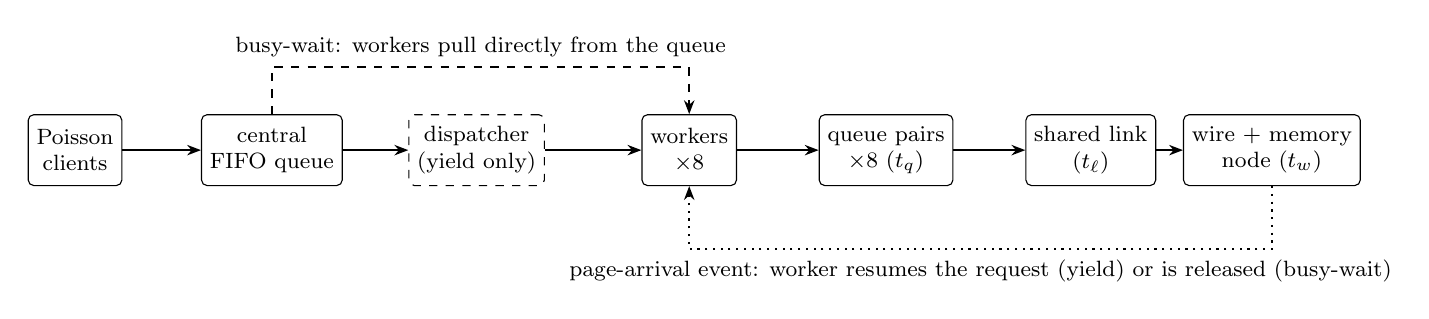
\begin{tikzpicture}[x=1cm,y=1cm,font=\footnotesize,
  box/.style={draw,rounded corners=2pt,minimum height=0.9cm,align=center,inner sep=3pt},
  arr/.style={-{Stealth[length=5pt]},thick}]
\node[box] (cl) at (0,0) {Poisson\\clients};
\node[box] (q) at (2.5,0) {central\\FIFO queue};
\node[box,dashed] (d) at (5.1,0) {dispatcher\\(yield only)};
\node[box] (w) at (7.8,0) {workers\\$\times 8$};
\node[box] (qp) at (10.3,0) {queue pairs\\$\times 8$ ($t_q$)};
\node[box] (lk) at (12.9,0) {shared link\\($t_\ell$)};
\node[box] (mem) at (15.2,0) {wire + memory\\node ($t_w$)};
\draw[arr] (cl)--(q); \draw[arr] (q)--(d); \draw[arr] (d)--(w); \draw[arr] (w)--(qp); \draw[arr] (qp)--(lk); \draw[arr] (lk)--(mem);
\draw[arr,dotted] (mem.south) -- ++(0,-0.8) -| node[pos=0.25,below]{page-arrival event: worker resumes the request (yield) or is released (busy-wait)} (w.south);
\draw[arr,dashed] (q.north) -- ++(0,0.6) -| node[pos=0.25,above]{busy-wait: workers pull directly from the queue} (w.north);
\end{tikzpicture}
\caption{Structure of the simulated compute node and of the RDMA path. Both policies share the queue and the RDMA model; they differ in how a worker behaves while a fetch is outstanding.}
\label{fig:arch}
\end{figure*}

\subsection{Request life cycle under the two policies}
Figure~\ref{fig:timeline} shows what a single worker does when it handles a remote miss. Under busy-waiting, the worker executes the first half of $t_c$, posts the fetch, then stays on the core doing nothing but polling the completion queue until the page lands---a total occupancy of $t_c + t_f$. Under yielding, the worker posts the fetch, pays one switch $t_s$ to hand control back to the scheduler, and picks up another request from its inbox. When the page eventually arrives, the suspended request gets priority over new arrivals; the worker pays a second switch to resume it, runs the remaining half of $t_c$, and completes. Local-hit requests follow the same code path in both systems.

\begin{figure}[t]
\centering
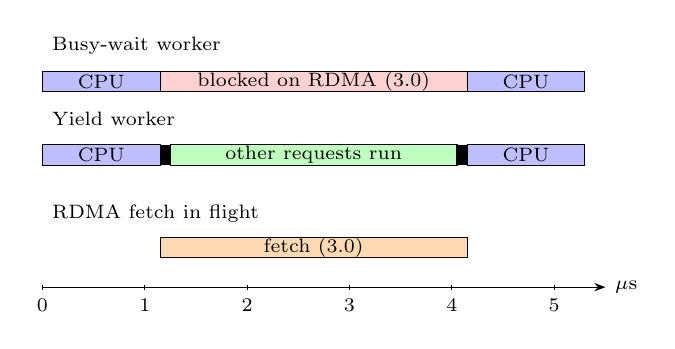
\begin{tikzpicture}[x=1.3cm,y=0.62cm,font=\scriptsize]
\def\hh{0.42}
\node[anchor=west] at (0,3.45) {Busy-wait worker};
\fill[blue!25] (0,2.5) rectangle (1.15,2.5+\hh); \draw (0,2.5) rectangle (1.15,2.5+\hh);
\fill[red!18] (1.15,2.5) rectangle (4.15,2.5+\hh); \draw (1.15,2.5) rectangle (4.15,2.5+\hh);
\fill[blue!25] (4.15,2.5) rectangle (5.3,2.5+\hh); \draw (4.15,2.5) rectangle (5.3,2.5+\hh);
\node at (0.575,2.71) {CPU}; \node at (2.65,2.71) {blocked on RDMA (3.0)}; \node at (4.725,2.71) {CPU};
\node[anchor=west] at (0,1.95) {Yield worker};
\fill[blue!25] (0,1.0) rectangle (1.15,1.0+\hh); \draw (0,1.0) rectangle (1.15,1.0+\hh);
\fill[black] (1.15,1.0) rectangle (1.25,1.0+\hh);
\fill[green!25] (1.25,1.0) rectangle (4.05,1.0+\hh); \draw (1.25,1.0) rectangle (4.05,1.0+\hh);
\fill[black] (4.05,1.0) rectangle (4.15,1.0+\hh);
\fill[blue!25] (4.15,1.0) rectangle (5.3,1.0+\hh); \draw (4.15,1.0) rectangle (5.3,1.0+\hh);
\node at (0.575,1.21) {CPU}; \node at (2.65,1.21) {other requests run}; \node at (4.725,1.21) {CPU};
\node[anchor=west] at (0,0.0) {RDMA fetch in flight};
\fill[orange!30] (1.15,-0.9) rectangle (4.15,-0.9+\hh); \draw (1.15,-0.9) rectangle (4.15,-0.9+\hh);
\node at (2.65,-0.69) {fetch (3.0)};
\draw[-{Stealth[length=4pt]}] (0,-1.5)--(5.5,-1.5) node[right]{$\mu$s};
\foreach \x in {0,1,2,3,4,5} {\draw (\x,-1.45)--(\x,-1.55) node[below]{\x};}
\end{tikzpicture}
\caption{One remote request on a worker (default parameters, switch widths exaggerated). The busy-wait worker is occupied for 5.3~$\mu$s; the yield worker for about 2.34~$\mu$s of its own time.}
\label{fig:timeline}
\end{figure}

\subsection{RDMA path}
Every worker owns one dedicated queue pair, modelled as a single-server FIFO with service time $t_q$. After leaving the queue pair, a command occupies the single shared link for $t_\ell$, then the page spends a fixed $t_w$ on the wire and in the remote memory node. An unloaded fetch therefore completes in $t_q + t_\ell + t_w = 3.0~\mu$s. This three-stage pipeline captures exactly the properties described in Section~\ref{sec:background}: fetches take a few microseconds on an idle fabric, commands on a single queue pair are ordered, and all queue pairs compete for a fixed aggregate link capacity. The link time $t_\ell = 0.5~\mu$s per page translates to roughly 65~Gb/s of page traffic, capping the network at two fetches per microsecond. The simulator maintains a per-queue-pair counter of outstanding fetches; this counter is the congestion signal the page-fault-aware dispatcher reads. For the sensitivity experiment in Section~\ref{sec:pf} we also test $t_q = 2.0~\mu$s with $t_w = 0.5~\mu$s, keeping the unloaded fetch unchanged but making the queue pair a larger share of the delay.

\subsection{The yield system}
A dispatcher process holds the central queue and assigns work to \emph{idle} workers---those with empty inboxes. Each worker's inbox is a priority store in which page-arrival resumptions (priority 0) beat new requests (priority 1). Three dispatch policies are implemented. Round-robin (RR) scans idle workers in a rotating order. Page-fault-aware dispatch (PF) selects, among idle workers, the one with the fewest outstanding fetches and breaks ties round-robin, as shown in Algorithm~\ref{alg:dispatch}.

Beyond those two baselines, we design and implement an \emph{Adaptive Hybrid} policy (\texttt{adaptive}). When a worker hits a page fault, it checks system queue pressure through the condition:
\begin{equation}
\label{eq:must_yield}
\text{must\_yield} = (|W.\text{inbox}| > 0) \lor (|Q| > 0) \lor (N_{\text{idle}} = 0)
\end{equation}
If $\text{must\_yield}$ is true---meaning work is queued or every other core is busy---the worker yields right away, posts an asynchronous RDMA fetch, and switches to the queued tasks to prevent head-of-line blocking. If $\text{must\_yield}$ is false---the system is idle with spare cores available---the worker spin-waits on the fetch directly. This avoids both the outgoing and incoming switches ($2t_s$ in total), recovering the light-load latency advantage of busy-waiting while preserving the high-load capacity benefit of yielding. The dispatcher is modelled as free of processor cost, a simplification that favours the yield system and is listed as a limitation in Section~\ref{sec:discussion}.

The number of requests simultaneously in flight is capped at $P = 4096$. This represents the fixed pool of 131{,}072 pre-allocated unithreads in Adios \cite{adios}, scaled down only to keep simulation time reasonable. Without a cap, the model allows an unbounded backlog of half-completed requests when load exceeds capacity, which distorted our earliest measurements (Section~\ref{sec:method}).

\subsection{Optional page-cache model}
By default, each request independently draws a hit or miss with probability $h$. To test whether this independence assumption matters, the simulator also supports a true LRU cache over $M = 100{,}000$ pages, with the cache holding a configurable fraction. Each request selects a page from a Zipf distribution with exponent $s$, so page $k$ is chosen with probability proportional to $k^{-s}$; $s = 0$ gives uniform access \cite{zipf}. A hit promotes the page to most-recently-used; a fetched page is inserted on arrival, evicting the least-recently-used page when the cache is full. The cache is pre-warmed with the most popular pages. Two simultaneous misses on the same page each issue a separate fetch, since request merging is not modelled.

\subsection{Capacity bounds}
\label{sec:bounds}
The model's structure permits a closed-form estimate of each policy's saturation throughput. We write $\Lambda$ for a capacity in MRPS.

\textbf{Busy-wait.} A worker is occupied for $t_L$ on a hit and for $t_c+t_f$ on a miss, so the mean occupancy is
\begin{equation}
S_{bw}=h\,t_L+(1-h)(t_c+t_f),
\label{eq:sbw}
\end{equation}
and the eight workers can complete at most
\begin{equation}
\Lambda_{bw}=N/S_{bw}.
\label{eq:lbw}
\end{equation}
With the defaults, $S_{bw}=4.41$~$\mu$s and $\Lambda_{bw}=1.81$~MRPS. Queueing in the shared link extends the real fetch time slightly beyond $t_f$, so the measured plateau should fall a little below this bound.

\textbf{Yield.} The processor time of a request is $h\,t_L+(1-h)(t_c+2t_s)$, because every miss pays two switches. Three resources can limit throughput:
\begin{align}
\Lambda_{cpu}&=\frac{N}{h\,t_L+(1-h)(t_c+2t_s)},\label{eq:lcpu}\\
\Lambda_{link}&=\frac{1}{(1-h)\,t_\ell},\label{eq:llink}\\
\Lambda_{qp}&=\frac{N}{(1-h)\,t_q}.\label{eq:lqp}
\end{align}
The yield system saturates at $\Lambda_{y}=\min(\Lambda_{cpu},\Lambda_{link},\Lambda_{qp})$. With the defaults the three values are 3.92, 2.50 and 10.0 MRPS. The shared link is therefore the bottleneck of the yield system at 2.50~MRPS, and the processors are only about 64\% busy at that point.

\textbf{Break-even rule.} When the link is not the limiting resource, comparing Equations~\eqref{eq:lbw} and~\eqref{eq:lcpu} gives a simple condition: yielding raises capacity if and only if
\begin{equation}
2\,t_s<t_f.
\label{eq:breakeven}
\end{equation}
In words, the two switches that a fault costs must take less time than the fetch they hide. With $t_f=3.0$~$\mu$s the threshold is $t_s=1.5$~$\mu$s.

\textbf{Efficiency view.} In the busy-wait system the useful fraction of occupied time is $(h\,t_L+(1-h)t_c)/S_{bw}=0.46$: more than half of the processor time at saturation is spent waiting. To carry the yield system's 2.50~MRPS, a busy-wait system would need $2.50\,S_{bw}\approx 11$ workers instead of eight, ignoring the link limit. These two figures are derived from the model equations, not measured in the simulator.

\section{Experimental Method}
\label{sec:method}

\subsection{Load generation and measurement}
Request arrivals follow a Poisson process whose rate equals the offered load. We deliberately use open-loop arrivals: a closed-loop client slows its request rate whenever the system slows down and thereby masks queueing delay, which is precisely what we want to observe \cite{leverich}. Each simulation run covers 200~ms of simulated time. The first 20~ms serve as a warm-up period and are excluded from all measurements, leaving a 180~ms measurement window. At 1.5~MRPS the window captures roughly 270{,}000 requests; at 0.5~MRPS, about 90{,}000.

\emph{Latency} for a request is defined as its completion time minus its arrival time, capturing everything: queueing, processor work, context switches, and the page-fetch wait. Percentiles are computed with linear interpolation over requests that both arrived after the warm-up and completed before the run ended. \emph{Throughput} is the count of completions inside the measurement window divided by the window length. A throughput value equal to the offered load means the system kept up; we treat such values as lower bounds on capacity and mark them in every table.

One limitation of this procedure is worth flagging. When the system is overloaded, requests that are still in queue at the end of the run have no completion time and are silently excluded from the latency sample. Latency values reported above capacity therefore understate the true delay and vary with the simulated duration. We include them to show where the saturation knee lies but do not interpret their absolute magnitude as a result.

\subsection{Experiments}
Table~\ref{tab:experiments} enumerates the experiments, the parameter each one varies, and the script and output file in the repository.\footnote{\url{https://github.com/Pradeepthi-P01/adios-simulation}} The main comparison runs the three policies (busy-wait, yield with RR dispatch, and yield with PF dispatch) at nine offered loads between 0.5 and 3.0~MRPS. All sweeps use the default parameters from Table~\ref{tab:params} except for the quantity under study.

\begin{table}[t]
\caption{Experiments and where to find them in the repository \texttt{adios-simulation}}
\label{tab:experiments}
\centering
\footnotesize
\begin{tabular}{p{2.5cm}p{2.6cm}p{2.0cm}}
\toprule
Experiment & Varied & Script \\
\midrule
Policy comparison & offered load 0.5--3.0 & \texttt{run\_experiments}, \texttt{plots} \\
PF vs.\ RR & load 1.8--2.4, $t_q\in\{1,2\}$ & \texttt{pf\_vs\_rr} \\
Hit-rate sweep & $h=0.1$--0.8 & \texttt{sweep\_hitrate} \\
Switch-cost sweep & $t_s=0.02$--4~$\mu$s & \texttt{sweep\_switchcost} \\
LRU cache + Zipf & skew $s$, cache size & \texttt{sweep\_cache} \\
Adaptive evaluation & load 0.2--2.5, $t_s=0.02$--1.5~$\mu$s & \texttt{sweep\_adaptive} \\
\bottomrule
\end{tabular}
\end{table}

All runs use the fixed seed 42, with one exception: the dispatch-rule comparison averages five seeds (1--5) because the effect of PF-aware dispatch is small and a single seed could easily be misleading. All other experiments are single runs. We did not compute confidence intervals; for that reason we describe differences of a few percent as small and stop short of calling them statistically significant.

\subsection{Implementation of the worker loops}
Algorithm~\ref{alg:workers} gives the logic of both worker types as implemented in the simulator. They differ in exactly one place: what the worker does between posting the fetch and completing the request. The busy-wait worker remains in that blocked state for the full fetch, while the yield worker pays a switch cost $t_s$, returns to its inbox, and may start other requests. Because the simulator is process-based, a ``fetch'' is itself a SimPy process that travels through the queue pair, the shared link, and the wire delay in sequence; in the yield system it deposits a resume message in the inbox of the issuing worker when it finishes.

\begin{algorithm}[t]
\caption{Worker behaviour in the simulator.}
\label{alg:workers}
\begin{algorithmic}[1]
\small
\Procedure{BusyWaitWorker}{}
\Loop
\State $r \gets$ next request from the central queue
\If{$r$ hits local memory} \State run $t_L$
\Else \State run $t_c/2$; \; \Call{Fetch}{$r$} and wait; \; run $t_c/2$
\EndIf
\State record completion of $r$
\EndLoop
\EndProcedure
\Procedure{YieldWorker}{}
\Loop
\State $m \gets$ next message in inbox (resumptions first)
\If{$m$ is a new request $r$}
\If{$r$ hits} \State run $t_L$; \; record completion
\ElsIf{adaptive $\land$ \Call{Uncontended}{}} \Comment{spin-wait}
\State run $t_c/2$; \; \Call{Fetch}{$r$} and wait; \; run $t_c/2$; \; record completion
\Else
\State run $t_c/2$; \; start \Call{Fetch}{$r$} in background
\State pay $t_s$ \Comment{yield}
\EndIf
\Else \Comment{page has arrived for $r$}
\State pay $t_s$; \; run $t_c/2$; \; record completion of $r$
\EndIf
\EndLoop
\EndProcedure
\end{algorithmic}
\end{algorithm}

\subsection{Reproducibility}
All simulation parameters are defined as named constants in \texttt{config.py}. The scripts should be run in the order \texttt{run\_experiments}, \texttt{plots}, \texttt{pf\_vs\_rr}, \texttt{sweep\_hitrate}, \texttt{sweep\_switchcost}, and \texttt{sweep\_cache}; each writes a CSV file and a figure to the \texttt{results} directory. Tables and figures in this paper are produced directly from those CSV files by two helper scripts distributed with the paper source, so no number in the main text is typed by hand---except for the derived quantities, which follow from the equations in Section~\ref{sec:bounds}. With a fixed seed, every run is deterministic.

\subsection{Corrections to our first version}
Checking the simulator's output against the capacity bounds of Section~\ref{sec:bounds} revealed two measurement errors in an earlier version. Both are corrected in the results reported here.

\emph{Throughput by arrival time.} The first version counted each request toward throughput at the moment it arrived, not when it completed. Near saturation, the growing backlog then inflated or deflated the apparent rate depending on where the measurement window ended. Switching to completion-time counting fixed this, and the busy-wait plateau stabilized at a constant 1.77~MRPS across all overloaded conditions.

\emph{Unbounded in-flight requests.} In the original yield model any number of requests could be started and left half-finished simultaneously. Above the link limit the simulator then reported throughputs above 2.50~MRPS (2.56 at 2.8~MRPS offered, 2.60 at 3.0~MRPS), which is physically impossible when the link carries at most two fetches per microsecond and 80\% of requests need one. Capping the pool at $P = 4096$ eliminated the effect, and the yield plateau settled at 2.50~MRPS, matching Equation~\eqref{eq:llink}.

Both errors would have inflated the apparent advantage of yielding at high load. We document them here because they illustrate why a plausible-looking graph still needs to be checked against an analytic bound.

\subsection{Validation}
We validate the simulator in three independent ways. First, at light load the measured median latency of 5.3~$\mu$s matches the expected $t_c + t_f$ exactly (Table~\ref{tab:main}). Second, the measured throughput plateaus are compared with the bounds from Equations~\eqref{eq:lbw}--\eqref{eq:lqp} across several hit rates and switch costs in Sections~\ref{sec:hit} and~\ref{sec:switch}. Third, the LRU cache with uniform access ($s = 0$) and a 20\% cache fraction must reproduce a 20\% hit rate, and it does (19.9\% in Table~\ref{tab:cache}).

\section{Results}
\label{sec:results}
Unless stated otherwise, the local hit probability is 20\%, the switch cost is 0.02~$\mu$s and all values come from the seed-42 runs described in Section~\ref{sec:method}. Latencies are in microseconds.

\subsection{Throughput under increasing load}
Figure~\ref{fig:tput} plots the carried throughput against the offered load. Up to 1.5~MRPS every policy carries the whole load. At 1.8~MRPS the busy-wait system already falls slightly short (1.77~MRPS) while the yield systems still carry 1.80. From there the curves separate. Busy-wait stays at 1.77~MRPS however much load is offered, which is 97.7\% of its bound $\Lambda_{bw}=1.81$~MRPS from Equation~\eqref{eq:lbw}. Yield follows the offered load up to 2.5~MRPS and then stays at 2.50~MRPS, which is its link bound from Equation~\eqref{eq:llink} to within 0.1\%. The ratio of the two plateaus is $2.497/1.772=1.41$. The two dispatch rules give identical throughput.

\begin{figure}[t]
\centering
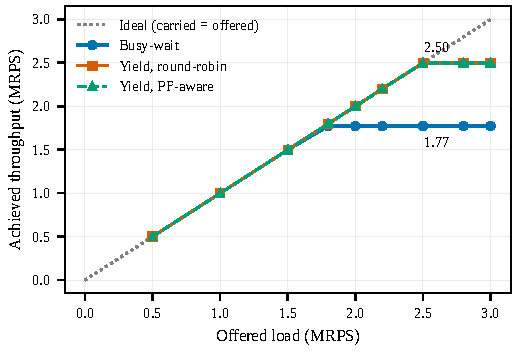
\includegraphics[width=\columnwidth]{tput}
\caption{Carried throughput against offered load for the three policies. The dotted line shows carried equal to offered.}
\label{fig:tput}
\end{figure}

\subsection{Tail latency}
Figure~\ref{fig:p999} shows the 99.9th percentile of latency, and Table~\ref{tab:main} gives the full set of percentiles. At 0.5~MRPS the policies are indistinguishable (6.5 and 6.6~$\mu$s at P99.9), and the median is 5.30 versus 5.32~$\mu$s, a difference of 0.02~$\mu$s that comes from the two extra switches of a miss. As the load rises, the busy-wait tail grows first. At 1.0~MRPS the P99.9 is 8.7~$\mu$s against 7.7 for yield. At 1.5~MRPS it is 17.2 against 8.9~$\mu$s, a factor of 1.93, and the P99 is 13.1 against 7.8~$\mu$s (1.68). At 1.8~MRPS busy-wait is past its capacity and the P99.9 jumps to about 3{,}000~$\mu$s, while yield has 10.6~$\mu$s. If a service-level target of 20~$\mu$s at P99.9 is assumed, busy-wait can carry about 1.5~MRPS (26.7~$\mu$s at 1.6) and yield about 2.2~MRPS (18.1~$\mu$s), a factor of roughly 1.5 in usable load.

\begin{figure}[t]
\centering
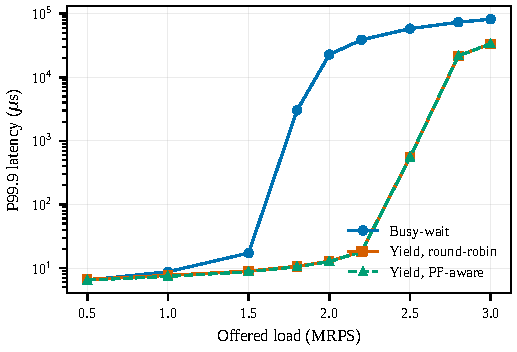
\includegraphics[width=\columnwidth]{p999}
\caption{99.9th percentile latency against offered load (log scale). Values above each policy's capacity understate the true delay (Section~\ref{sec:method}).}
\label{fig:p999}
\end{figure}

\begin{figure}[t]
\centering
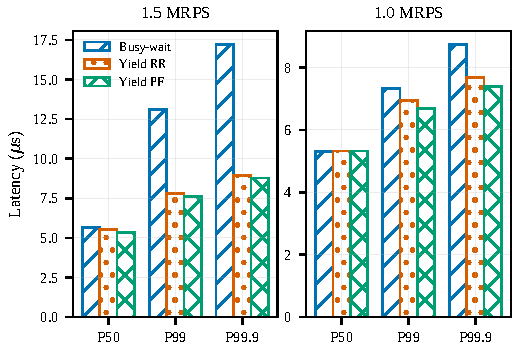
\includegraphics[width=\columnwidth]{bars}
\caption{Latency percentiles of the three policies at 1.0 and 1.5~MRPS.}
\label{fig:bars}
\end{figure}

The yield system keeps its P99.9 under 20~$\mu$s until 2.2~MRPS and reaches 552~$\mu$s at 2.5~MRPS, the load at which the link is exactly full. Above 2.5~MRPS both policies are overloaded and their latencies depend on how long the run lasts, so they are not comparable results. The PF-aware variant is almost the same as round-robin here (8.8 against 8.9~$\mu$s at 1.5~MRPS), which Section~\ref{sec:pf} examines.

\begin{table*}[t]
\caption{Throughput (MRPS) and latency ($\mu$s) of the three policies. The last column is the P99.9 of the PF-aware yield system.}
\label{tab:main}
\centering
\footnotesize
\begin{tabular}{r|rrrr|rrrr|r}
\toprule
 & \multicolumn{4}{c|}{Busy-wait} & \multicolumn{4}{c|}{Yield, round-robin} & PF-aware \\
Offered & Tput & P50 & P99 & P99.9 & Tput & P50 & P99 & P99.9 & P99.9 \\
\midrule
0.5 & 0.50 & 5.3 & 6.0 & 6.5 & 0.50 & 5.3 & 6.1 & 6.6 & 6.5 \\
1.0 & 1.00 & 5.3 & 7.3 & 8.7 & 1.00 & 5.3 & 6.9 & 7.7 & 7.4 \\
1.5 & 1.50 & 5.7 & 13.1 & 17.2 & 1.50 & 5.5 & 7.8 & 8.9 & 8.8 \\
1.8 & 1.77 & 1{,}626.7 & 2{,}948.4 & 3{,}014.3 & 1.80 & 5.8 & 9.0 & 10.6 & 10.5 \\
2.0 & 1.77 & 12{,}597.8 & 22{,}470.9 & 22{,}685.0 & 2.00 & 6.0 & 10.4 & 12.8 & 12.7 \\
2.2 & 1.77 & 21{,}786.2 & 38{,}449.5 & 38{,}787.7 & 2.20 & 6.4 & 13.9 & 18.1 & 18.0 \\
2.5 & 1.77 & 33{,}194.4 & 57{,}631.3 & 58{,}113.1 & 2.50 & 94.2 & 536.0 & 551.8 & 551.8 \\
2.8 & 1.77 & 42{,}476.4 & 72{,}710.2 & 73{,}297.4 & 2.50 & 11{,}460.3 & 21{,}461.4 & 21{,}708.8 & 21{,}708.7 \\
3.0 & 1.77 & 47{,}802.0 & 81{,}094.1 & 81{,}733.1 & 2.50 & 18{,}238.9 & 33{,}217.5 & 33{,}580.3 & 33{,}580.3
\\
\bottomrule
\end{tabular}
\end{table*}

\subsection{Effect of the local hit rate}
\label{sec:hit}
Figure~\ref{fig:hit} and Table~\ref{tab:hit} show the peak throughput when the local hit rate varies from 10\% to 80\%. The offered load is 4.0~MRPS, so any value equal to 4.0 is a lower bound. For hit rates where neither system is capped the ratio of yield to busy-wait is 1.37 at 10\%, 1.41 at 20\% and 1.51 at 40\%. It is therefore not largest at low hit rates, which is where a first reading of the argument for yielding might place it. The bound ratio explains why: the yield ceiling $1/((1-h)t_\ell)$ and the busy-wait ceiling $N/S_{bw}$ both rise as $h$ grows, but the second rises more slowly while it is not yet limited by the processors. At 60\% the yield system is cut off by the offered load (4.0 against a bound of 5.0), so the measured ratio of 1.35 is only a lower bound; the bounds themselves give 5.00/3.04, about 1.64. At 80\% both systems reach the offered load and show no difference.

\begin{figure}[t]
\centering
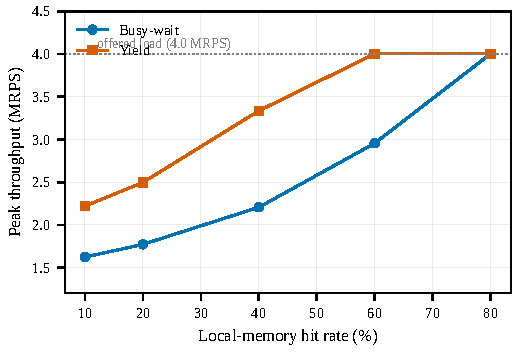
\includegraphics[width=\columnwidth]{hit}
\caption{Peak throughput against the local hit rate, with an offered load of 4.0~MRPS.}
\label{fig:hit}
\end{figure}

\begin{table}[t]
\caption{Hit-rate sweep: analytic bound and measured peak (MRPS). $^{\dagger}$ capped by the offered load of 4.0~MRPS.}
\label{tab:hit}
\centering
\footnotesize
\setlength{\tabcolsep}{3pt}
\begin{tabular}{r|rrr|rrr|r}
\toprule
 & \multicolumn{3}{c|}{Busy-wait} & \multicolumn{3}{c|}{Yield} & Ratio \\
$h$ (\%) & Bound & Meas. & \% & Bound & Meas. & \% & Y/B \\
\midrule
10 & 1.648 & 1.623 & 98.5 & 2.222 & 2.220 & 99.9 & 1.37 \\
20 & 1.814 & 1.772 & 97.7 & 2.500 & 2.497 & 99.9 & 1.41 \\
40 & 2.273 & 2.206 & 97.1 & 3.333 & 3.336 & 100.1 & 1.51 \\
60 & 3.042 & 2.956 & 97.2 & 4.000$^{\dagger}$ & 4.003 & 100.1 & $\geq$1.35 \\
80 & 4.000$^{\dagger}$ & 4.004 & 100.1 & 4.000$^{\dagger}$ & 4.003 & 100.1 & 1.00$^{\dagger}$
\\
\bottomrule
\end{tabular}
\end{table}

The column marked ``\%'' compares measurement with bound. For busy-wait the measured peak is 97.1--98.5\% of the bound in all uncapped rows, with the shortfall caused by queueing in the link, and for yield it is 99.9--100.1\%. The simple formulas of Section~\ref{sec:bounds} therefore describe the simulator well.

In the Adios paper, reducing local memory from the full working set down to a tenth of it costs the yield-based system 25\% of its throughput and the busy-wait system 60\% \cite{adios}. Our model does not reproduce that pattern. Between 40\% and 10\% hit rate the busy-wait peak falls by 26\% (2.21 to 1.62) and the yield peak by 33\% (3.34 to 2.22), because the link ceiling of the yield system is inversely proportional to the miss rate. The offered-load cap prevents a comparison over the paper's full range, so we make no claim about the 100\%--10\% interval.

\subsection{Page-fault-aware dispatch}
\label{sec:pf}
Table~\ref{tab:pf} and Figure~\ref{fig:pfgain} compare the P99.9 latency of the two dispatch rules, averaged over five seeds, at loads between 1.8 and 2.4~MRPS and for both queue-pair settings. The PF-aware rule is better at nine of the ten points, by 0.09\% to 1.22\%, with an average gain of 0.61\% for $t_q=1$~$\mu$s and 0.51\% for $t_q=2$~$\mu$s. The gain is largest at the lowest load tested and shrinks as the load approaches the link limit; at 2.4~MRPS with $t_q=2$~$\mu$s the sign reverses ($-0.12$\%), which is the size of the noise in these runs.

\begin{table}[t]
\caption{P99.9 latency ($\mu$s, mean of five seeds) of round-robin (RR) and PF-aware dispatch.}
\label{tab:pf}
\centering
\footnotesize
\begin{tabular}{llrrr}
\toprule
Setting & Load & RR & PF & Gain (\%) \\
\midrule
QP 1.0 & 1.8 & 10.87 & 10.73 & +1.22 \\
QP 1.0 & 2.0 & 13.28 & 13.17 & +0.81 \\
QP 1.0 & 2.2 & 18.60 & 18.50 & +0.57 \\
QP 1.0 & 2.3 & 25.20 & 25.11 & +0.37 \\
QP 1.0 & 2.4 & 42.86 & 42.82 & +0.09 \\
QP 2.0 & 1.8 & 10.95 & 10.83 & +1.17 \\
QP 2.0 & 2.0 & 13.36 & 13.26 & +0.78 \\
QP 2.0 & 2.2 & 18.61 & 18.55 & +0.32 \\
QP 2.0 & 2.3 & 25.22 & 25.12 & +0.42 \\
QP 2.0 & 2.4 & 42.85 & 42.90 & -0.12
\\
\bottomrule
\end{tabular}
\end{table}

\begin{figure}[t]
\centering
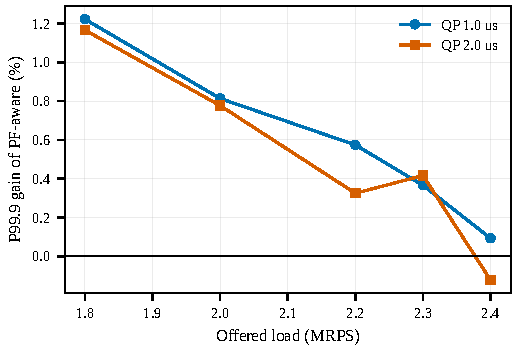
\includegraphics[width=\columnwidth]{pfgain}
\caption{Gain of PF-aware over round-robin dispatch in P99.9 latency, in percent.}
\label{fig:pfgain}
\end{figure}

The published gain is larger: up to 7.5\% for Memcached and 27\% for RocksDB \cite{adios}. A likely reason for the difference follows from the model. At 2.5~MRPS each queue pair handles 0.25 fetches per microsecond, which keeps it 25\% busy for $t_q=1$ and 50\% busy for $t_q=2$, while the shared link is 100\% busy. The dispatcher can move fetches between queue pairs but cannot reduce the load on the link, so the delay that it could remove is small. Real queue pairs have burstier arrivals and variable service times, which our fixed-time model lacks. We have not tested this explanation with a modified model, so it is a hypothesis.

\subsection{Cost of a context switch}
\label{sec:switch}
Figure~\ref{fig:switch} and Table~\ref{tab:switch} vary the cost $t_s$ of one switch from 0.02 to 4~$\mu$s. For $t_s\le0.5$~$\mu$s the yield peak is 2.50~MRPS, the link bound, because the processors still have spare capacity. For larger costs the processors become the bottleneck and the peak follows $\Lambda_{cpu}$, falling to 2.21 at 1~$\mu$s, 1.81 at 1.5~$\mu$s and 0.95~MRPS at 4~$\mu$s. By linear interpolation the throughput of yield and busy-wait are equal at $t_s\approx1.57$~$\mu$s, which agrees with the break-even rule $t_s<t_f/2=1.5$~$\mu$s of Equation~\eqref{eq:breakeven} (the small excess comes from the 2.3\% by which the real busy-wait plateau lies under its bound). For the tail at 1.5~MRPS, yield stays below busy-wait's 17.2~$\mu$s up to about 1.44~$\mu$s.

Both reported switch costs for user-level threads---0.02~$\mu$s (40 cycles) for Adios's unithreads and 0.10~$\mu$s (191 cycles) for Shinjuku \cite{adios}---fall comfortably below this 1.5~$\mu$s ceiling. In contrast, standard kernel-space context switching takes $\approx 4~\mu$s \cite{adios}, driving yield capacity down to 0.95~MRPS (merely 54\% of spinning throughput). This confirms the paper's core thesis: yielding's feasibility in disaggregated paging hinges entirely on keeping thread-switch overhead below microsecond scales.

\begin{figure*}[t]
\centering
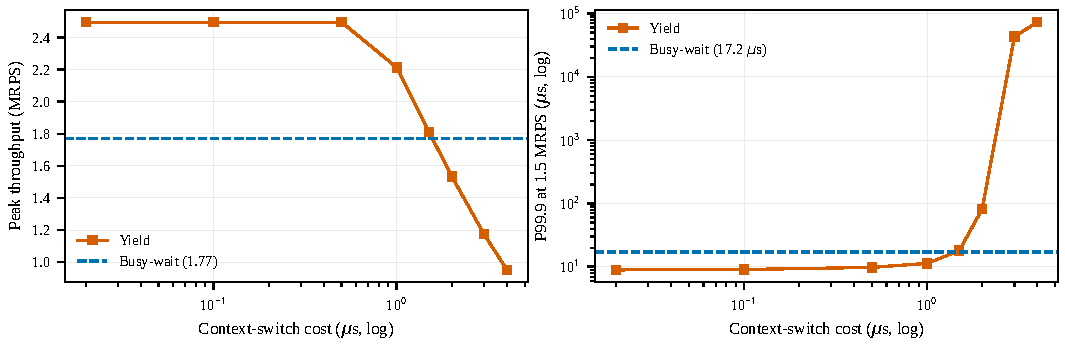
\includegraphics[width=0.92\textwidth]{switch}
\caption{Effect of the context-switch cost on the yield system. Left: peak throughput. Right: P99.9 latency at 1.5~MRPS. Dashed lines show busy-wait.}
\label{fig:switch}
\end{figure*}

\begin{table}[t]
\caption{Switch-cost sweep: analytic yield bound and measured peak (MRPS), and P99.9 at 1.5~MRPS ($\mu$s).}
\label{tab:switch}
\centering
\footnotesize
\begin{tabular}{rrrrr}
\toprule
$t_s$ ($\mu$s) & Bound & Meas. & \% & P99.9 \\
\midrule
0.02 & 2.500 & 2.497 & 99.9 & 8.9 \\
0.1 & 2.500 & 2.497 & 99.9 & 9.1 \\
0.5 & 2.500 & 2.497 & 99.9 & 9.8 \\
1 & 2.216 & 2.214 & 99.9 & 11.3 \\
1.5 & 1.814 & 1.813 & 99.9 & 18.0 \\
2 & 1.536 & 1.535 & 100.0 & 82.0 \\
3 & 1.175 & 1.174 & 99.9 & 43133.5 \\
4 & 0.951 & 0.951 & 100.0 & 73011.6
\\
\bottomrule
\end{tabular}
\end{table}

\subsection{Realistic hit rates: LRU cache and skewed access}
\label{sec:cache}
The fixed 20\% hit probability is a simplification, since real hit rates come from cache size and access skew. Table~\ref{tab:cache} reports the LRU model of Section~\ref{sec:model} with an offered load of 5.0~MRPS. First, uniform access ($s=0$) with a 20\% cache produces a hit rate of 19.9\% and the same throughputs as the fixed model (1.77 and 2.50~MRPS), which validates the shortcut. Second, skew raises the hit rate sharply: 31.8\% at $s=0.5$, 59.3\% at $s=0.8$ and 80.6\% at $s=0.99$. With it both throughputs rise and the ratio grows from 1.41 to 1.67 at a hit rate of 59\%. This matches the 1.64 predicted from the bounds at the same hit rate (5.0/3.04 is the bound ratio at 60\%) and agrees with the corresponding row of the hit-rate sweep. Third, a larger cache has the same effect as more skew (Figure~\ref{fig:cache}): at $s=0.8$ the yield peak grows from 3.08 to 4.87~MRPS as the cache grows from 5\% to 20\% of the pages. Rows marked $^{\ddagger}$ equal the offered load and carry no ratio.

\begin{table}[t]
\caption{LRU cache with Zipf access: hit rate and peak throughput (MRPS). $^{\ddagger}$ equals the offered load of 5.0~MRPS (read as ``at least'').}
\label{tab:cache}
\centering
\footnotesize
\begin{tabular}{rrrrr}
\toprule
Skew / size & Hit (\%) & Busy-wait & Yield & Ratio \\
\midrule
\multicolumn{5}{l}{\textit{Skew sweep (cache 20\%)}} \\
0 & 19.9 & 1.77 & 2.50 & 1.41 \\
0.5 & 31.8 & 2.00 & 2.90 & 1.45 \\
0.8 & 59.3 & 2.92 & 4.87 & 1.67 \\
0.99 & 80.6 & 4.56 & 5.01$^{\ddagger}$ & $\geq$1.10 \\
1.2 & 94.8 & 5.01$^{\ddagger}$ & 5.01$^{\ddagger}$ & -- \\
\multicolumn{5}{l}{\textit{Size sweep (skew 0.8)}} \\
5\% & 36.2 & 2.12 & 3.08 & 1.45 \\
10\% & 46.5 & 2.41 & 3.68 & 1.53 \\
20\% & 59.3 & 2.92 & 4.87 & 1.67 \\
40\% & 75.2 & 3.96 & 5.01$^{\ddagger}$ & $\geq$1.26 \\
60\% & 85.9 & 5.01$^{\ddagger}$ & 5.01$^{\ddagger}$ & --
\\
\bottomrule
\end{tabular}
\end{table}

\begin{figure*}[t]
\centering
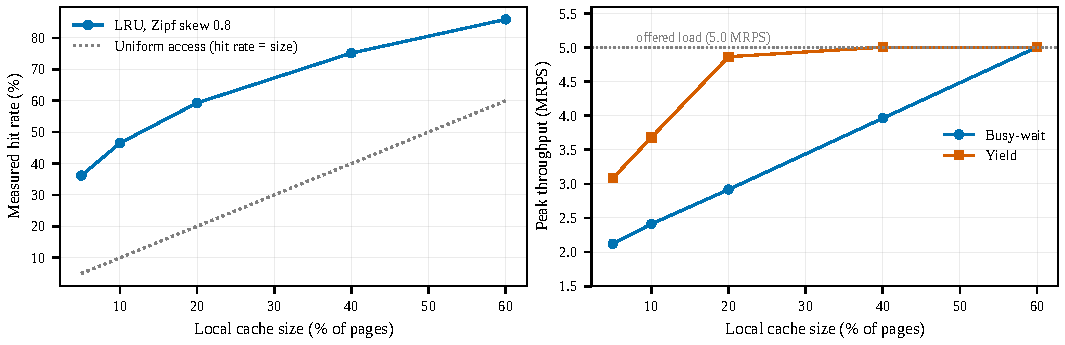
\includegraphics[width=0.92\textwidth]{cache}
\caption{LRU cache with Zipf skew 0.8. Left: measured hit rate against cache size. Right: peak throughput against cache size.}
\label{fig:cache}
\end{figure*}

\begin{figure}[t]
\centering
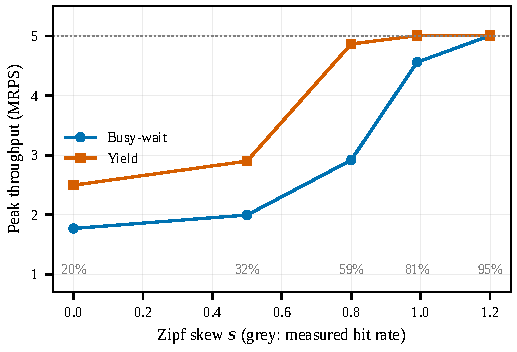
\includegraphics[width=\columnwidth]{skew}
\caption{Peak throughput against Zipf skew for a 20\% cache. Grey numbers are the measured hit rates.}
\label{fig:skew}
\end{figure}

\subsection{Load-Aware Adaptive Hybrid Yielding}
\label{sec:adaptive}
Evaluating pure spinning against pure yielding exposes an inherent tension across load regimes. Under light traffic ($< 1.0$~MRPS), processor cores sit idle between request arrivals. Unconditionally yielding on every miss forces the system to pay a 40~ns round-trip context-switch penalty ($2 \times 0.02~\mu$s) even though no other task is waiting for the CPU, giving busy-waiting a slight latency edge (5.30~$\mu$s vs.\ 5.32~$\mu$s median). If thread switches are slower ($t_s \ge 0.5~\mu$s), this light-load penalty swells to 28\% at $t_s = 1.5~\mu$s. Conversely, under heavy traffic ($> 1.5$~MRPS), spinning suffers from severe HOL blocking: worker cores stall waiting on RDMA packets, capping throughput at 1.77~MRPS and causing tail latency ($P_{99.9}$) to jump from 17.2~$\mu$s to over 3{,}000~$\mu$s.

To resolve this dilemma, we evaluate our \emph{Load-Aware Adaptive Hybrid Yielding} policy (\texttt{sweep\_adaptive.py}). Workers consult the local condition in Equation~\eqref{eq:must_yield} during fault handling: if work is queued locally, in the central dispatcher, or if peer cores are saturated, the worker yields immediately to prevent blocking. Otherwise, it polls locally on the RDMA completion queue.

\begin{figure*}[t]
\centering
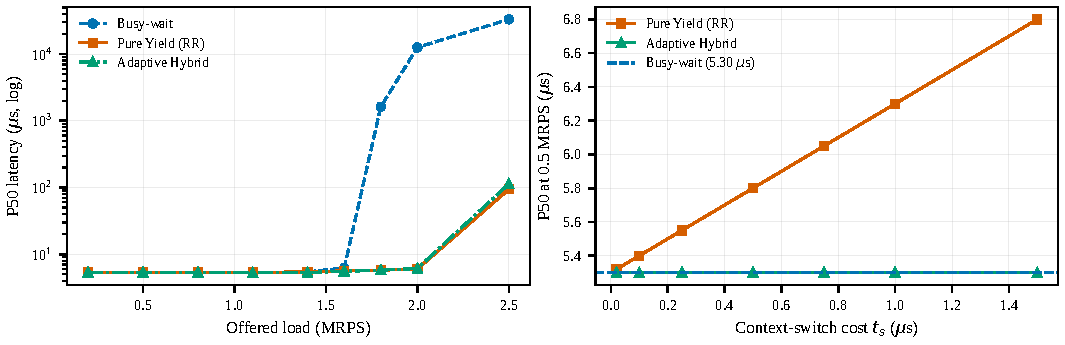
\includegraphics[width=0.92\textwidth]{adaptive}
\caption{Performance of the Load-Aware Adaptive Hybrid Yielding strategy. Left: median latency ($P_{50}$) across offered loads (0.2--2.5~MRPS). Right: sensitivity of median latency ($P_{50}$) to context-switch cost $t_s$ at light load (0.5~MRPS).}
\label{fig:adaptive}
\end{figure*}

\begin{table*}[t]
\caption{Performance of Load-Aware Adaptive Hybrid Yielding compared to Busy-Wait and Pure Yield (RR) across offered loads (0.2--2.5~MRPS). Throughput in MRPS, latencies in $\mu$s.}
\label{tab:adaptive}
\centering
\footnotesize
\begin{tabular}{r|rrr|rrr|rrr}
\toprule
 & \multicolumn{3}{c|}{Busy-wait} & \multicolumn{3}{c|}{Pure Yield (RR)} & \multicolumn{3}{c}{Adaptive Hybrid (Ours)} \\
Offered & Tput & P50 & P99.9 & Tput & P50 & P99.9 & Tput & P50 & P99.9 \\
\midrule
0.2 & 0.20 & 5.3 & 6.0 & 0.20 & 5.3 & 6.0 & 0.20 & 5.3 & 6.0 \\
0.5 & 0.50 & 5.3 & 6.5 & 0.50 & 5.3 & 6.6 & 0.50 & 5.3 & 8.0 \\
0.8 & 0.80 & 5.3 & 7.8 & 0.80 & 5.3 & 7.3 & 0.80 & 5.3 & 9.8 \\
1.1 & 1.10 & 5.3 & 9.4 & 1.10 & 5.3 & 7.9 & 1.10 & 5.3 & 10.8 \\
1.4 & 1.40 & 5.4 & 13.3 & 1.40 & 5.4 & 8.6 & 1.40 & 5.3 & 11.9 \\
1.6 & 1.60 & 6.2 & 26.7 & 1.60 & 5.6 & 9.4 & 1.60 & 5.5 & 13.3 \\
1.8 & 1.77 & 1{,}626.7 & 3{,}014.3 & 1.80 & 5.8 & 10.6 & 1.80 & 5.8 & 15.5 \\
2.0 & 1.77 & 12{,}597.8 & 22{,}685.0 & 2.00 & 6.0 & 12.8 & 2.00 & 6.1 & 18.8 \\
2.5 & 1.77 & 33{,}194.4 & 58{,}113.1 & 2.50 & 94.2 & 551.8 & 2.50 & 113.4 & 972.9
\\
\bottomrule
\end{tabular}
\end{table*}

Figure~\ref{fig:adaptive} and Table~\ref{tab:adaptive} highlight three core outcomes:
\begin{enumerate}
\item \emph{Eliminating the Light-Load Tax}: Between 0.2 and 1.1~MRPS, Adaptive Hybrid achieves $P_{50} = 5.30~\mu$s, matching busy-waiting exactly and saving the 20~ns unneeded switch. At 1.4~MRPS, Adaptive achieves $5.32~\mu$s, outperforming both busy-wait ($5.44~\mu$s) and pure yield ($5.43~\mu$s).
\item \emph{Avoiding High-Load Saturation}: At 1.8~MRPS, busy-wait collapses to $P_{50} = 1{,}626.7~\mu$s and $P_{99.9} = 3{,}014.3~\mu$s. Adaptive detects queuing instantly, maintaining $1.80$~MRPS at $P_{50} = 5.77~\mu$s and scaling smoothly to the 2.50~MRPS link bound.
\item \emph{Switch-Cost Resilience}: Figure~\ref{fig:adaptive} (right) tracks 0.5~MRPS median latency as switch cost $t_s$ varies from 0.02 to 1.5~$\mu$s. While pure yield degrades from 5.32 to 6.80~$\mu$s (+28\% slowdown), Adaptive Hybrid stays flat at 5.30~$\mu$s across the entire range by recognizing that cores are free and avoiding the scheduler.
\end{enumerate}

\subsection{Comparison with the published results}
\label{sec:paperlink}
Table~\ref{tab:paperlink} sets the simulator's results beside the figures that the Adios paper reports for its microbenchmark and applications. The two agree on the direction of every effect that the simulator can express. The size of the throughput gain is somewhat smaller in the simulator (1.41 against 1.58 for the microbenchmark), and the busy-wait plateau is higher (1.77 against about 1.4~MRPS). The second difference is expected: the per-request times of 0.85 and 5.3~$\mu$s that we take from the paper predict a plateau of 1.81~MRPS for eight workers, yet the authors measured about 1.4. The real system therefore spends time outside those figures, plausibly in networking and dispatching, and our model omits that time. We cannot confirm this from the simulator. The remaining rows of Table~\ref{tab:paperlink} are not reproduced or not testable, and we mark them as such.

\begin{table*}[t]
\caption{Published results of Adios \cite{adios} against this simulation study. ``Derived'' values are computed from the simulator's results and the model equations.}
\label{tab:paperlink}
\centering
\footnotesize
\begin{tabular}{p{4.6cm}p{4.7cm}p{4.6cm}p{2.4cm}}
\toprule
Quantity & Adios paper & This study & Agreement \\
\midrule
Busy-wait throughput plateau & about 1.4~MRPS (DiLOS) & 1.77~MRPS & differs \\
Yield throughput plateau & grows to about 2.5~MRPS & 2.50~MRPS (link bound) & matches \\
Peak throughput gain from yielding & 1.58$\times$ over DiLOS & 1.41$\times$ & same direction \\
P99.9 gain near the busy-wait knee & 2.83$\times$ at 1.3~MRPS & 1.93$\times$ at 1.5~MRPS & same direction \\
Link use at the busy-wait plateau & about 50\% & 71\% (derived) & same direction \\
Link use at the yield plateau & up to 82\% & 100\% (by construction) & same direction \\
Gain of PF-aware dispatch (P99.9) & up to 7.5\% (Memcached), 27\% (RocksDB) & at most 1.2\% & much smaller \\
Penalty of yielding at low load & about 6\% higher P99.9 at 0.2~MRPS & about 2\% at 0.5~MRPS (single run) & same direction \\
Loss of throughput when local memory shrinks & yield 25\%, busy-wait 60\% (100\% to 10\% local) & yield 33\%, busy-wait 26\% (40\% to 10\%) & not reproduced \\
Preemptive scheduling instead of yield & no benefit & not modelled & not tested \\
\bottomrule
\end{tabular}
\end{table*}

\section{Analytical Extrapolation}
\label{sec:analysis}
The capacity formulas of Section~\ref{sec:bounds} reproduce the simulated plateaus to within 3\% in every configuration we ran. That accuracy makes it reasonable to use them for questions that the simulator was not asked. Everything in this section is computed from the equations with the default parameters of Table~\ref{tab:params}. \emph{None of it was simulated}, so it is a prediction of the model and not a measurement. For the busy-wait policy we now also apply the link bound of Equation~\eqref{eq:llink}, which never binds at the default settings but does when more workers are added. The yield bound is $\Lambda_y$ as defined earlier.

\subsection{How many workers does each policy need?}
Solving the capacity equations for $N$ gives the number of workers that a policy needs to carry a load $\Lambda$ when the network is not the limit:
\begin{equation}
N_{bw}(\Lambda)=\Lambda\,S_{bw},\qquad N_{y}(\Lambda)=\Lambda\bigl(h\,t_L+(1-h)(t_c+2t_s)\bigr).
\label{eq:needed}
\end{equation}
Table~\ref{tab:workers} evaluates the two expressions. To carry 2.5~MRPS, the ceiling of the yield system, a spinning system would need 11.0 workers while a yielding system needs 5.1, which is a ratio of 2.2. Put differently, the eight workers of the simulated node are about 64\% busy at the yield ceiling, so the remaining capacity could be given to other tasks or to a smaller machine. We stress that these are capacity figures. A real system has to run below 100\% utilization to keep its tail latency bounded, as Figure~\ref{fig:p999} shows, so a deployment would add some margin to every entry.

\begin{table}[t]
\caption{Workers needed to carry a load, from Equation~\eqref{eq:needed} (derived, not simulated).}
\label{tab:workers}
\centering
\footnotesize
\begin{tabular}{rrr}
\toprule
Load (MRPS) & Busy-wait & Yield \\
\midrule
1.5 & 6.6 & 3.1 \\
2.0 & 8.8 & 4.1 \\
2.5 & 11.0 & 5.1 \\
\bottomrule
\end{tabular}
\end{table}

Figure~\ref{fig:scale}(a) illustrates how saturation scales with core count. The yield curve climbs steeply with $N$ until hitting the network bottleneck at $N \approx 5.1$ workers, plateauing thereafter because the 100~GbE link cannot serialize more pages. The busy-wait curve scales with core count more gradually, taking $N \approx 11$ workers to reach that same link ceiling. This reveals a critical architectural insight: yielding provides the biggest efficiency dividend when CPU cores are scarce relative to link bandwidth. At 4 cores, yielding offers $2.16\times$ higher capacity; at 8 cores, $1.38\times$; and beyond 11 cores, both policies saturate the physical link equally. Adios evaluated only $N=8$, so this scaling cross-over is an original prediction of our model.

\subsection{Sensitivity to the fetch time}
The busy-wait capacity depends on the fetch time because a spinning worker is occupied for all of it, whereas the yield capacity at the link limit does not. Figure~\ref{fig:scale}(b) varies the unloaded fetch time $t_f$ from 2 to 6~$\mu$s with every other parameter fixed. The predicted capacity ratio is 1.13 at 2~$\mu$s, 1.38 at the default 3~$\mu$s, 1.63 at 4~$\mu$s, 1.88 at 5~$\mu$s and 2.13 at 6~$\mu$s. The break-even switch cost of Equation~\eqref{eq:breakeven} rises in step, from 1.0 to 3.0~$\mu$s. Both trends say the same thing: the slower the remote memory, the more there is to gain by hiding it. The lower end of the range (2--3~$\mu$s) is the one reported for a 4~KiB read on a 100~GbE card \cite{adios}. Larger values would correspond to a more distant memory node, a congested fabric or a slower technology, and the model suggests that yielding becomes more attractive in each of those cases. This reading agrees with the motivation of the original paper, although neither it nor our simulator tests it directly.

\begin{figure*}[t]
\centering
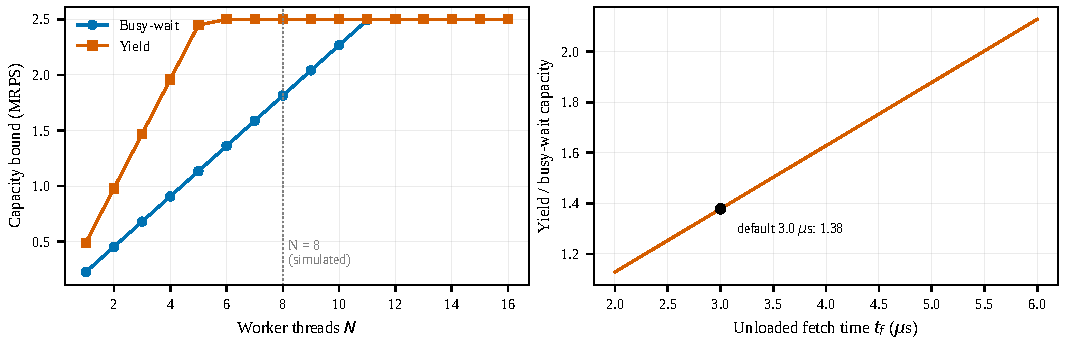
\includegraphics[width=0.92\textwidth]{scale}
\caption{Analytical predictions (not simulated). (a) Capacity bound against the number of workers for $h=20\%$. (b) Ratio of the yield capacity to the busy-wait capacity against the unloaded fetch time, for $N=8$.}
\label{fig:scale}
\end{figure*}

\subsection{Concurrency of fetches}
Little's law relates the average number of fetches in flight to the completion rate and the time each fetch takes. At the plateau of the busy-wait system, 1.77~MRPS with 80\% of requests missing and a fetch of at least 3.0~$\mu$s, there are on average at least $1.77\times0.8\times3.0\approx4.2$ fetches outstanding, out of at most eight. The yield system at 2.50~MRPS carries at least $2.50\times0.8\times3.0=6.0$, which is 0.75 per queue pair. Because queueing at the link lengthens each fetch beyond its unloaded time, both figures are lower bounds. They show that the spinning system leaves almost half of its possible fetch slots empty on average, and that the yield system uses more of them with the same number of workers. This is the quantitative form of the under-utilization argument that Section~\ref{sec:background} gave in words, and it again agrees with the direction reported for the real system, where the link utilization rises from about 50\% to 82\% \cite{adios}.

\subsection{Summary of the Predictions}
In summary, our analytical model yields three concrete takeaways:
\begin{enumerate}
\item \emph{Hardware footprint}: Yielding achieves target throughput with under half the physical cores required by busy-waiting under default parameters (5.1 vs.\ 11.0 workers for 2.5~MRPS).
\item \emph{Sensitivity to network delay}: Slower remote fetch times widen yielding's throughput advantage over spinning, making yielding increasingly attractive on congested or multi-hop networks.
\item \emph{Break-even threshold}: Yielding's throughput advantage disappears whenever thread context switching exceeds $t_f / 2 = 1.5~\mu$s, explaining why kernel-level paging must spin while unikernel unithreads can yield.
\end{enumerate}

\section{Discussion}
\label{sec:discussion}

\subsection{Key Empirical and Analytical Insights}
Our simulation results align closely with the mathematical models, establishing three primary takeaways. First, yielding fundamentally relocates the performance bottleneck from compute cores to the network fabric. Because busy-waiting pins cores for the entire duration of a remote fetch, 8 worker cores cap throughput at 1.77~MRPS even though the 100~GbE link can carry substantially more. By freeing cores to continue processing local requests and issuing subsequent fetches, yielding drives system throughput to the physical 2.50~MRPS link bound. Second, yielding prevents early queue buildup below saturation: at 1.5~MRPS, yielding cuts P99.9 tail latency roughly in half compared to spinning. Third, the advantage relies strictly on microsecond-scale context switching; the inequality $2t_s < t_f$ serves as a practical litmus test for whether yielding is worth implementing on a given system.

From a resource provisioning perspective, busy-waiting wastes over half (54\%) of active core cycles spinning idly on RDMA completions at saturation. Matching the 2.50~MRPS throughput of an 8-worker yielding node would require approximately 11 spinning cores, representing a substantial hardware overhead.

\subsection{Pathologies of Pure Yielding and the Hybrid Solution}
Our sensitivity sweeps demonstrate that pure yielding is not universally optimal:
\begin{enumerate}
\item \emph{High Context-Switch Latency}: When thread switching exceeds $t_s \approx 1.5~\mu$s, context-switch overhead outweighs the fetch duration, driving yielding throughput below spinning.
\item \emph{Light Workload Penalties}: At low arrival rates, cores are largely idle. Yielding on every miss incurs two context switches ($2 \times 0.02 = 0.04~\mu$s) without providing any concurrency benefit, adding an unnecessary 20~ns latency overhead. In systems with slower thread packages, this overhead expands to several microseconds.
\item \emph{High Cache Hit Rates}: When local hit rates reach 80\%, page faults become infrequent, causing spinning and yielding to converge to identical performance ceilings.
\end{enumerate}

Our \emph{Load-Aware Adaptive Hybrid Yielding} policy eliminates these drawbacks. By checking queue occupancy locally before deciding to yield, workers spin when the server is uncongested and switch only when backlog accumulates. This provides the low latency of spinning at light load, the high saturation throughput of yielding under stress, and complete immunity to context-switch degradation up to $t_s = 1.5~\mu$s.

\subsection{Explaining Divergences from Published Adios Data}
Table~\ref{tab:paperlink} details the points of comparison between our simulation and the published Adios paper. While both agree on qualitative trends, numerical values diverge in three specific areas:
\begin{itemize}
\item \emph{Busy-wait saturation}: Adios reported $\approx 1.4$~MRPS on its microbenchmark, whereas our simulator yields 1.77~MRPS. This is expected because real-world NIC doorbell ringing and lock contention add overheads not captured in our two fixed CPU service times.
\item \emph{PF-aware dispatch gain}: Adios achieved up to 7.5\% (Memcached) and 27\% (RocksDB) tail latency improvements from congestion-aware dispatching, whereas our model observes $\le 1.2\%$. Real RDMA fabrics experience bursty arrivals and variable service times where queue imbalance is pronounced; in our deterministic-time model, the shared link remains the dominant bottleneck, leaving little per-QP delay for the dispatcher to eliminate.
\item \emph{Memory pressure degradation}: Real OS paging incurs lock contention, frame allocation stalls, and synchronous writebacks under memory pressure, which explains why Adios's measured throughput dropped faster when DRAM shrank.
\end{itemize}

\subsection{Assumptions and Threats to Validity}
To maintain focus on core scheduling dynamics, our model makes several simplifying assumptions:
\begin{itemize}
\item \textbf{Deterministic service latencies}: CPU and network delays are modeled as fixed constants rather than stochastic distributions, which likely compresses the tail compared to real systems.
\item \textbf{Idealized dispatcher}: The central dispatcher runs with zero CPU overhead and infinite throughput, abstracting away central lock contention that would limit scalability beyond 10--12 cores.
\item \textbf{Absence of reclaimer and prefetcher}: Free page frames are assumed to be immediately available; we do not model page eviction delays or multi-page prefetching pipelines.
\item \textbf{Unmerged page requests}: Concurrent misses to the same page produce duplicate RDMA fetches rather than merging into a single transfer.
\item \textbf{Finite in-flight pool}: We cap concurrent in-flight requests at 4,096 to prevent memory leaks during overload, which is smaller than Adios's 131,072 pool.
\end{itemize}

\subsection{Methodological Reflections}
During development, comparing simulation plateaus against closed-form bounds caught two significant implementation bugs: an arrival-timestamp windowing error that distorted saturation throughput, and an unbounded request pool that allowed physically impossible link throughputs ($>2.50$~MRPS). Deriving simple capacity equations proved essential for verifying simulation correctness before interpreting graphs.

\subsection{Directions for Future Research}
Several extensions would build naturally on this study. Simulating variable core counts ($N = 2$--16) and remote fetch times ($t_f = 2$--6~$\mu$s) would directly validate our analytical predictions. Incorporating heavy-tailed request service times and stochastic network jitter would better capture tail effects. Finally, evaluating dispatcher CPU overhead and implementing a multi-queue decentralized dispatcher would test scalability limits for modern 64-core and 128-core servers.

\section{Conclusion}
\label{sec:conclusion}
This work examined one specific claim of the Adios paper---that yielding during a remote page fetch outperforms spinning once context-switch cost is small---by constructing a discrete-event simulator and validating it against closed-form capacity bounds. With a 20\% local hit rate, our experiments showed that yielding lifts peak throughput from 1.77 to 2.50~MRPS (a factor of 1.41) and roughly halves the 99.9th percentile latency at 1.5~MRPS. The fundamental reason in both cases is that the yield system's ceiling is the network link, while the busy-wait system's ceiling is its processor pool---the same explanation the original paper offers. Yielding loses its advantage when two context switches together cost as much as one fetch, which in our configuration happens at $t_s = 1.5~\mu$s, roughly 75 times larger than the switch cost of a unithread design. Using the capacity formulas as a predictive model rather than just a check, we find that yielding needs fewer than half as many workers as spinning to carry 2.5~MRPS (5.1 versus 11.0) and that its advantage grows with fetch time---a prediction we did not test with the simulator. The page-fault-aware dispatch rule helped by at most 1.2\% in our model, far below the gains the original system reports, and our memory-shrink experiment did not reproduce the published throughput-loss pattern.

Going beyond the reproduction exercise, we identified a fundamental weakness of pure yielding: it wastes context-switch budget when the system is lightly loaded and becomes sensitive to rising switch costs in environments without unithread-style scheduling. To address this, we introduced \emph{Load-Aware Adaptive Hybrid Yielding}, which dynamically switches between spin-polling when uncontended and yielding when queue pressure builds. The result is the best of both worlds: the median latency of spinning (5.30~$\mu$s) at light load, the saturation throughput (2.50~MRPS) and tail protection of yielding at heavy load, and complete immunity to context-switch cost increases up to 1.5~$\mu$s.

The simulator does not reproduce Adios---it omits the unikernel, unithread layout, polling delegation, reclaimer, and real network hardware, using fixed service times throughout. Its results are therefore best understood as evidence about the scheduling mechanism itself and as a convenient tool for identifying break-even operating points, rather than as predictions of absolute performance on real hardware. All code, result files, and figures are available in the project repository so that every number in this report can be independently regenerated.


\section*{Appendix: Derivation of the Capacity Bounds}
\label{sec:appendix}
Below we derive the formulas behind Equations~\eqref{eq:sbw}--\eqref{eq:breakeven} and verify the arithmetic against the default parameter values.

\textbf{Busy-wait occupancy.} A request is a local hit with probability $h$, in which case it occupies a worker for $t_L$. With probability $1-h$ it is a remote miss and the worker is held for both halves of the CPU work plus the entire fetch, giving $t_c + t_f$ assuming no network queueing. Averaging over both cases yields Equation~\eqref{eq:sbw}. Over a long run, the $N$ workers collectively deliver $N$ worker-microseconds per real microsecond, and each completed request consumes $S_{bw}$ of those, so the completion rate cannot exceed $N/S_{bw}$. Plugging in the defaults: $S_{bw} = 0.2 \times 0.85 + 0.8 \times 5.3 = 0.17 + 4.24 = 4.41~\mu$s, giving $8 / 4.41 = 1.814$~MRPS.

\textbf{Yield occupancy.} A hit still costs $t_L$. For a miss, the worker is busy only during computation: $t_c$ of CPU work in total, plus one switch away when the fetch is posted and one switch back when the page arrives. The fetch wait itself is off the critical path for the worker. Occupancy is therefore $h\,t_L + (1-h)(t_c + 2t_s)$. With the defaults: $0.17 + 0.8 \times 2.34 = 2.042~\mu$s, so $\Lambda_{cpu} = 8 / 2.042 = 3.918$~MRPS.

\textbf{Link and queue-pair limits.} Only misses consume network bandwidth, and each fetch holds the shared link for $t_\ell$. The link can pass at most $1/t_\ell$ pages per microsecond, capping the request rate at $1 / ((1-h)\,t_\ell) = 1 / (0.8 \times 0.5) = 2.5$~MRPS. Misses also spread over $N$ queue pairs, each handling one command per $t_q$, giving $N / ((1-h)\,t_q) = 8 / 0.8 = 10$~MRPS. The binding constraint is the smallest of the three---2.5~MRPS from the link.

\textbf{Break-even.} The two policies have equal per-request occupancy when $t_c + t_f = t_c + 2t_s$, that is, $t_s = t_f / 2$. For switch costs below this threshold, the yield system needs less worker time per request and therefore carries more load per core. The empirical crossover sits at approximately 1.57~$\mu$s, slightly above $t_f/2 = 1.5~\mu$s, because the measured busy-wait plateau of 1.77~MRPS is 2.3\% below its analytic bound. Solving $\Lambda_{cpu} = 1.772$ for $t_s$ gives 1.565~$\mu$s, consistent with the value found by interpolation in Section~\ref{sec:switch}.

\textbf{Median latency at light load.} At 0.5~MRPS the system is far from saturation and queueing is negligible. Since 80\% of requests are misses, the median request is a miss. It runs $t_c = 2.3~\mu$s of processor work and waits 3.0~$\mu$s for the page, completing in 5.3~$\mu$s. The simulator reports 5.30~$\mu$s for busy-wait and 5.32~$\mu$s for yield; the 0.02~$\mu$s gap is precisely the second context switch. This check verifies the service-time parameters independently of any queueing dynamics.


\section*{Acknowledgment}
The authors thank the course instructor for guidance on the scope of the project. The simulator and all result files are available in the project repository listed in Table~\ref{tab:experiments}.

\begin{thebibliography}{00}
\bibitem{adios} W. Yoon, J. Ok, S. Moon, and Y. Kwon, ``Adios to busy-waiting for microsecond-scale memory disaggregation,'' in \textit{Proc. 20th European Conf. on Computer Systems (EuroSys '25)}, Rotterdam, The Netherlands, Mar. 2025, doi: 10.1145/3689031.3717475.
\bibitem{dilos} W. Yoon, J. Ok, J. Oh, S. Moon, and Y. Kwon, ``DiLOS: Do not trade compatibility for performance in memory disaggregation,'' in \textit{Proc. 18th European Conf. on Computer Systems (EuroSys '23)}, Rome, Italy, 2023, pp. 266--282, doi: 10.1145/3552326.3567488.
\bibitem{infiniswap} J. Gu, Y. Lee, Y. Zhang, M. Chowdhury, and K. G. Shin, ``Efficient memory disaggregation with Infiniswap,'' in \textit{Proc. 14th USENIX Symp. on Networked Systems Design and Implementation (NSDI '17)}, Boston, MA, USA, 2017, pp. 649--667.
\bibitem{fastswap} E. Amaro, C. Branner-Augmon, Z. Luo, A. Ousterhout, M. K. Aguilera, A. Panda, S. Ratnasamy, and S. Shenker, ``Can far memory improve job throughput?'' in \textit{Proc. 15th European Conf. on Computer Systems (EuroSys '20)}, Heraklion, Greece, 2020, Art. 14, doi: 10.1145/3342195.3387522.
\bibitem{hermit} Y. Qiao, C. Wang, Z. Ruan, A. Belay, Q. Lu, Y. Zhang, M. Kim, and G. H. Xu, ``Hermit: Low-latency, high-throughput, and transparent remote memory via feedback-directed asynchrony,'' in \textit{Proc. 20th USENIX Symp. on Networked Systems Design and Implementation (NSDI '23)}, Boston, MA, USA, 2023, pp. 181--198.
\bibitem{leap} H. A. Maruf and M. Chowdhury, ``Effectively prefetching remote memory with Leap,'' in \textit{Proc. USENIX Annual Technical Conf. (USENIX ATC '20)}, 2020.
\bibitem{aifm} Z. Ruan, M. Schwarzkopf, M. K. Aguilera, and A. Belay, ``AIFM: High-performance, application-integrated far memory,'' in \textit{Proc. 14th USENIX Symp. on Operating Systems Design and Implementation (OSDI '20)}, 2020, pp. 315--332.
\bibitem{semeru} C. Wang, H. Ma, S. Liu, Y. Li, Z. Ruan, K. Nguyen, M. D. Bond, R. Netravali, M. Kim, and G. H. Xu, ``Semeru: A memory-disaggregated managed runtime,'' in \textit{Proc. 14th USENIX Symp. on Operating Systems Design and Implementation (OSDI '20)}, 2020, pp. 261--280.
\bibitem{shinjuku} K. Kaffes, T. Chong, J. T. Humphries, A. Belay, D. Mazi\`eres, and C. Kozyrakis, ``Shinjuku: Preemptive scheduling for $\mu$second-scale tail latency,'' in \textit{Proc. 16th USENIX Symp. on Networked Systems Design and Implementation (NSDI '19)}, Boston, MA, USA, 2019, pp. 345--360.
\bibitem{concord} R. Iyer, M. Unal, M. Kogias, and G. Candea, ``Achieving microsecond-scale tail latency efficiently with approximate optimal scheduling,'' in \textit{Proc. 29th Symp. on Operating Systems Principles (SOSP '23)}, Koblenz, Germany, 2023, pp. 466--481, doi: 10.1145/3600006.3613136.
\bibitem{zygos} G. Prekas, M. Kogias, and E. Bugnion, ``ZygOS: Achieving low tail latency for microsecond-scale networked tasks,'' in \textit{Proc. 26th Symp. on Operating Systems Principles (SOSP '17)}, Shanghai, China, 2017, pp. 325--341, doi: 10.1145/3132747.3132780.
\bibitem{shenango} A. Ousterhout, J. Fried, J. Behrens, A. Belay, and H. Balakrishnan, ``Shenango: Achieving high CPU efficiency for latency-sensitive datacenter workloads,'' in \textit{Proc. 16th USENIX Symp. on Networked Systems Design and Implementation (NSDI '19)}, Boston, MA, USA, 2019, pp. 361--378.
\bibitem{persephone} H. M. Demoulin, J. Fried, I. Pedisich, M. Kogias, B. T. Loo, L. T. X. Phan, and I. Zhang, ``When idling is ideal: Optimizing tail-latency for heavy-tailed datacenter workloads with Pers\'ephone,'' in \textit{Proc. 28th ACM Symp. on Operating Systems Principles (SOSP '21)}, 2021, pp. 621--637, doi: 10.1145/3477132.3483571.
\bibitem{caladan} J. Fried, Z. Ruan, A. Ousterhout, and A. Belay, ``Caladan: Mitigating interference at microsecond timescales,'' in \textit{Proc. 14th USENIX Symp. on Operating Systems Design and Implementation (OSDI '20)}, 2020, pp. 281--297.
\bibitem{capriccio} R. von Behren, J. Condit, F. Zhou, G. C. Necula, and E. Brewer, ``Capriccio: Scalable threads for Internet services,'' \textit{ACM SIGOPS Oper. Syst. Rev.}, vol. 37, no. 5, Oct. 2003, doi: 10.1145/1165389.945471.
\bibitem{arachne} H. Qin, Q. Li, J. Speiser, P. Kraft, and J. Ousterhout, ``Arachne: Core-aware thread management,'' in \textit{Proc. 13th USENIX Symp. on Operating Systems Design and Implementation (OSDI '18)}, Carlsbad, CA, USA, 2018, pp. 145--160.
\bibitem{sa} T. E. Anderson, B. N. Bershad, E. D. Lazowska, and H. M. Levy, ``Scheduler activations: Effective kernel support for the user-level management of parallelism,'' in \textit{Proc. 13th ACM Symp. on Operating Systems Principles (SOSP '91)}, Pacific Grove, CA, USA, 1991, pp. 95--109, doi: 10.1145/121132.121151.
\bibitem{unikernels} A. Madhavapeddy and D. J. Scott, ``Unikernels: The rise of the virtual library operating system,'' \textit{Commun. ACM}, vol. 57, no. 1, pp. 61--69, Jan. 2014, doi: 10.1145/2541883.2541895.
\bibitem{osv} A. Kivity, D. Laor, G. Costa, P. Enberg, N. Har'El, D. Marti, and V. Zolotarov, ``OSv---Optimizing the operating system for virtual machines,'' in \textit{Proc. USENIX Annual Technical Conf. (USENIX ATC '14)}, Philadelphia, PA, USA, 2014, pp. 61--72.
\bibitem{unikraft} S. Kuenzer \textit{et al.}, ``Unikraft: Fast, specialized unikernels the easy way,'' in \textit{Proc. 16th European Conf. on Computer Systems (EuroSys '21)}, 2021, pp. 376--394, doi: 10.1145/3447786.3456248.
\bibitem{ukl} A. Raza \textit{et al.}, ``Unikernel Linux (UKL),'' in \textit{Proc. 18th European Conf. on Computer Systems (EuroSys '23)}, Rome, Italy, 2023, pp. 590--605, doi: 10.1145/3552326.3587458.
\bibitem{conga} M. Alizadeh \textit{et al.}, ``CONGA: Distributed congestion-aware load balancing for datacenters,'' in \textit{Proc. ACM SIGCOMM}, Chicago, IL, USA, 2014, pp. 503--514, doi: 10.1145/2619239.2626316.
\bibitem{plb} M. A. Qureshi \textit{et al.}, ``PLB: Congestion signals are simple and effective for network load balancing,'' in \textit{Proc. ACM SIGCOMM}, Amsterdam, The Netherlands, 2022, pp. 207--218, doi: 10.1145/3544216.3544226.
\bibitem{killer} L. Barroso, M. Marty, D. Patterson, and P. Ranganathan, ``Attack of the killer microseconds,'' \textit{Commun. ACM}, vol. 60, no. 4, pp. 48--54, Apr. 2017, doi: 10.1145/3015146.
\bibitem{tail} J. Dean and L. A. Barroso, ``The tail at scale,'' \textit{Commun. ACM}, vol. 56, no. 2, pp. 74--80, Feb. 2013, doi: 10.1145/2408776.2408794.
\bibitem{tales} J. Li, N. K. Sharma, D. R. K. Ports, and S. D. Gribble, ``Tales of the tail: Hardware, OS, and application-level sources of tail latency,'' in \textit{Proc. ACM Symp. on Cloud Computing (SoCC)}, 2014, pp. 1--14.
\bibitem{kalia} A. Kalia, M. Kaminsky, and D. G. Andersen, ``Design guidelines for high performance RDMA systems,'' in \textit{Proc. USENIX Annual Technical Conf. (USENIX ATC '16)}, Denver, CO, USA, 2016, pp. 437--450.
\bibitem{leverich} J. Leverich and C. Kozyrakis, ``Reconciling high server utilization and sub-millisecond quality-of-service,'' in \textit{Proc. 9th European Conf. on Computer Systems (EuroSys '14)}, Amsterdam, The Netherlands, 2014, Art. 4, doi: 10.1145/2592798.2592821.
\bibitem{zipf} L. Breslau, P. Cao, L. Fan, G. Phillips, and S. Shenker, ``Web caching and Zipf-like distributions: Evidence and implications,'' in \textit{Proc. IEEE INFOCOM}, 1999, pp. 126--134.
\bibitem{cxl} CXL Consortium, ``Compute Express Link.'' [Online]. Available: \url{https://www.computeexpresslink.org}
\bibitem{simpy} Team SimPy, ``SimPy: Discrete event simulation for Python.'' [Online]. Available: \url{https://simpy.readthedocs.io}
\bibitem{adioscode} ANLAB-KAIST, ``Adios source code.'' [Online]. Available: \url{https://github.com/ANLAB-KAIST/adios}
\end{thebibliography}

\end{document}
